\documentclass[10pt,a4paper]{article}
\usepackage[utf8]{inputenc}
\usepackage[T1]{fontenc}
\usepackage{graphicx}
\usepackage{booktabs}
\usepackage{geometry}
\usepackage{hyperref}
\usepackage{times}
\usepackage{setspace}
\usepackage{enumitem}
\usepackage{caption}
\usepackage{float}
\usepackage{xcolor}
\usepackage{longtable}
\usepackage{array}
\usepackage{multicol}
\usepackage{tcolorbox}
\geometry{margin=2.0cm}

\definecolor{primaryblue}{HTML}{1A3C6E}
\definecolor{accentred}{HTML}{B91C1C}
\definecolor{warnamber}{HTML}{D97706}
\definecolor{notegray}{HTML}{4B5563}
\definecolor{lightbg}{HTML}{F0F4F8}
\definecolor{parch}{HTML}{FAF7F0}
\definecolor{novelrow}{HTML}{FEF3C7}

\title{\textbf{Mission Definition and Requirements for a Conceptual Reusable Launch Vehicle (CRLV-1): \\ A Sustainable, Reusability-Driven Design Framework}\\[0.4em]
\large v1.0 (refined)}
\author{Research Team \\ \small Tsinghua Summer Program on AI Co-Design of Reusable Rockets}
\date{18 July 2026}

\begin{document}

\maketitle

% Executive summary box
\begin{tcolorbox}[colback=parch,colframe=primaryblue,arc=2pt,boxrule=1pt]
\centering\textbf{Executive Summary}\\[0.3em]
\begin{tabular}{lll}
\toprule
\textbf{Parameter} & \textbf{Threshold / Goal} & \textbf{v1.0 fix} \\
\midrule
L0-01 Payload & 1,200 / 2,000 kg (LEO 500 / SSO 700 km) & --- \\
L0-02 Reuses  & 10 / 20 flights, refurb $<$ 15\% & --- \\
L0-03 Cost    & $<$ \$3,500 / \$2,500 per kg & relaxed from \$2,800 (small-vehicle disadvantage) \\
L0-04 Sustainability & $<$ 15 t CO\textsubscript{2}e/t payload & GRI = Payload / [E\textsubscript{flight} + E\textsubscript{refurb}] (unit-consistent) \\
L0-05 Responsiveness & 30 / 14 days & --- \\
L0-06 Reliability & compound $\geq 0.95$ (10 flights) & implies per-flight $\geq 0.994$ / 0.997 \\
\bottomrule
\end{tabular}
\end{tcolorbox}

\vspace{1em}

\begin{abstract}
\noindent This paper presents the mission definition and Level-0 / Level-1 requirements for \textbf{CRLV-1}, a conceptual partially reusable launch vehicle targeting 1{,}200--2{,}000~kg of payload to low Earth orbit (LEO) or sun-synchronous orbit (SSO). The work draws on a structured review of 2025--2026 reusable launch vehicle (RLV) developments, with particular attention to the rapid emergence of Chinese state and commercial programmes. A defining feature of the framework is the explicit, \textbf{unit-consistent} definition of a Green Reusability Index (GRI) and a formal requirement to evaluate sea-based net-capture recovery as an alternative to conventional propulsive landing. Where public 2025--2026 sources disagree on the precise designation of the Chinese booster that demonstrated net-capture in 2026 (variously described as Long March 10, 10B, or 12A), the document uses the conservative family label \textit{Long March 10/12A} and flags the naming uncertainty. All quantitative claims are either cross-referenced to a 2025--2026 source or explicitly labelled as \textit{estimate} or \textit{illustrative}; in particular, no fabricated numerical comparison of GRI is presented---the framework figure shows the data inputs and a unit-consistent definition, with quantitative values to be produced during the Day-7 multi-objective optimisation. A self-critical review identified twelve issues in the original draft; all twelve are addressed in this refined v1.0.
\end{abstract}

\tableofcontents
\vspace{1em}

%==================================================================
\section{Introduction}
%==================================================================
The rapid maturation of reusable launch vehicle (RLV) technology, led by SpaceX's Falcon~9 and accelerated by Chinese state and commercial programmes in 2025--2026, has fundamentally changed the economics of access to space. As of mid-2026, multiple Chinese vehicles have either achieved or attempted first-stage recovery, with a publicly reported demonstration of a sea-based \textbf{net-capture} architecture on a Chinese methalox booster representing a noteworthy first for the Chinese orbital-class programme \cite{arstechnica2026}. Public sources disagree on the precise designation of that vehicle, variously referring to it as \textit{Long March 10}, \textit{Long March 10B}, or \textit{Long March 12A}; the present document uses the conservative family label \textit{Long March 10/12A} throughout and flags the naming uncertainty explicitly in the references and risk register (R08).

This paper documents the Day-1 mission-definition process for \textbf{CRLV-1} (Conceptual Reusable Launch Vehicle 1), an academic, demonstrator-class RLV positioned in the payload gap between small dedicated launchers (e.g., Rocket Lab Electron, $\sim$300~kg) and medium-lift reusable vehicles (e.g., Falcon~9, $\sim$22.8~t). The framework integrates performance, reusability, cost, and sustainability considerations; introduces the GRI as a primary figure of merit; and explicitly retains a propulsive-vs-net-capture recovery trade for the Day-6 deep-dive.

%==================================================================
\section{Research Methodology and Data Sources}
%==================================================================
A systematic literature and news review was conducted on 2025--2026 RLV developments. Primary public sources included SpaceNews, Ars Technica, Global Times, China-in-Space, manufacturer press releases, and market analyses. Quantitative claims were cross-verified against at least two independent sources wherever possible; values that could not be cross-verified are explicitly flagged as \textit{estimate}.

\begin{table}[H]
\centering
\caption{Reference vehicles analysed (reusable configuration unless noted).}
\label{tab:refs}
\small
\begin{tabular}{@{}p{4.0cm}p{2.5cm}p{2.8cm}p{6.7cm}@{}}
\toprule
\textbf{Vehicle} & \textbf{Operator} & \textbf{LEO payload (reusable, kg)} & \textbf{Status / note} \\
\midrule
Falcon 9 Block 5        & SpaceX            & 22,800    & Operational, $>$20 flights per booster, propulsive landing. \\
New Glenn               & Blue Origin       & 45,000    & Maiden flight 2025; methalox; 7~m fairing. \\
Zhuque-3                & Landspace (CN)    & $\sim$18,300 & Stainless-steel methalox; maiden orbital Dec 2025 (recovery failed). \\
\textbf{Long March 10/12A}* & CASC (CN)     & 12,000 (est.) & \textit{*}Designation uncertain; sea-based net-capture 2026. \\
Hyperbola-3             & iSpace (CN)       & 8,500     & Kerolox; maiden slipped to 2026; dedicated drone-ship. \\
Pallas-1                & Galactic Energy (CN) & 8,000   & Kerolox; first flight 2026. \\
\midrule
\textit{CRLV-1 (proposed)} & This work      & \textbf{1,200--2,000} & \textit{Conceptual demonstrator; methalox; recovery TBD.} \\
\bottomrule
\end{tabular}
\end{table}

Sustainability data were drawn from recent life-cycle assessment (LCA) studies, which consistently indicate that traditional RP-1/LOX systems produce 15--20~t CO\textsubscript{2}e per tonne of payload delivered to LEO \cite{lca2024,lca2025}. The mid-point value of $\sim$19~t CO\textsubscript{2}e/t used in this document is illustrative within that published range, not a precise measurement.

%==================================================================
\section{Mission Statement and Top-Level (L0) Objectives}
%==================================================================
\textbf{Mission Statement.} Develop CRLV-1, a conceptual partially reusable launch vehicle capable of delivering 1{,}200--2{,}000~kg of payload to LEO or SSO with at least 10 first-stage reuses, a competitive recurring cost, and explicit lifecycle sustainability performance.

\textbf{Level-0 Objectives (with threshold/goal split):}
\begin{enumerate}[leftmargin=*]
    \item \textbf{Payload delivery (L0-01).} 1,200~kg threshold / 2,000~kg goal to 500~km LEO or 700~km SSO, single-flight success $\geq 0.98$ (implies compound $\geq 0.95$ over 10 flights; consistent with L0-06).
    \item \textbf{Reusability (L0-02).} First stage reusable for $\geq 10$ flights (threshold) / $\geq 20$ flights (goal), with refurbishment cost $< 15\%$ of new-build cost.
    \item \textbf{Cost efficiency (L0-03).} Recurring launch cost target $< \$3{,}500$/kg (threshold) and $< \$2{,}500$/kg (goal). \textit{The threshold is set $\sim$30\% above the current Falcon~9 effective rate to reflect the inherent scale disadvantage of a $\sim$1.5~t class vehicle; an aggressive $\$2{,}800$/kg value used in earlier drafts is flagged as \textbf{likely optimistic} and demoted to a stretch goal.}
    \item \textbf{Sustainability (L0-04).} Lifecycle CO\textsubscript{2}-equivalent emissions per tonne of payload delivered to be $< 15$~t CO\textsubscript{2}e/t (threshold), a $\sim$20\% reduction against the $\sim$19~t CO\textsubscript{2}e/t RP-1 baseline.
    \item \textbf{Responsiveness (L0-05).} Capable of launch within 30 days (threshold) / 14 days (goal) of payload integration for dedicated missions.
    \item \textbf{Reliability (L0-06).} Compound mission success $\geq 0.95$ over the first 10 flights; this implies per-flight success $\geq 0.994$ at the threshold and $\geq 0.997$ at the goal, which is at the upper edge of historical new-booster performance.
\end{enumerate}

%==================================================================
\section{Key Requirements Hierarchy (L1)}
%==================================================================
A structured Level-1 (L1) requirements breakdown was developed with explicit verification methods. The full set is summarised in Table~\ref{tab:L1}; novel elements are highlighted.

\begin{table}[H]
\centering
\caption{Selected Level-1 requirements for CRLV-1 (Day-1 draft, 14 L1 requirements).}
\label{tab:L1}
\small
\begin{tabular}{@{}p{1.5cm}p{4.8cm}p{2.4cm}p{2.4cm}p{3.0cm}@{}}
\toprule
\textbf{ID} & \textbf{Requirement} & \textbf{Threshold} & \textbf{Goal} & \textbf{Verification} \\
\midrule
L1-P01 & Payload to 500~km LEO (reusable) & 1,200~kg & 2,000~kg & Trajectory sim. \\
L1-P02 & Injection accuracy (alt / incl) & $\pm$20~km / $\pm$0.05$^{\circ}$ & $\pm$10~km / $\pm$0.02$^{\circ}$ & Flight test + GNC \\
\rowcolor{novelrow}L1-P03 & Fairing internal volume (v1.0 fix) & $\varnothing 3.4$~m $\times 6.5$~m & $\varnothing 3.6$~m $\times 7.0$~m & Inspection \\
\addlinespace
L1-R01 & Per-flight recovery success & $\geq 0.90$ & $\geq 0.98$ & Flight test + MC \\
L1-R02 & Number of reuses per first stage & 10 & 20 & Ops tracking \\
\rowcolor{novelrow}L1-R03 & Recovery: propulsive OR net-capture & Trade closed Day 6 & --- & Trade study \\
\addlinespace
L1-C01 & Recurring launch cost per flight & $\leq \$4.2$~M & $\leq \$3.0$~M & Cost model (Day 8) \\
L1-C02 & Refurb cost fraction of new-build & $\leq 15\%$ & $\leq 10\%$ & Cost model \\
\addlinespace
L1-E01 & Propellant preference & LOX/LCH\textsubscript{4} & + bio-CH\textsubscript{4} option & Lifecycle assessment \\
\rowcolor{novelrow}L1-E02 & Green Reusability Index (GRI) as FoM & $\geq 1.20 \times$ F9 (illus.) & $\geq 1.35 \times$ F9 (illus.) & Day 7 model \\
\addlinespace
L1-S01 & Compound success, first 10 flights & $\geq 0.95$ & $\geq 0.97$ & RBD + MC \\
L1-O01 & Compatible launch site & Hainan (Wenchang) & + Jiuquan sea-zone & CONOPS \\
L1-O02 & Dedicated + rideshare modes & Yes & Yes & ICD \\
\rowcolor{novelrow}L1-O03 & Landing accuracy (propulsive) & $\pm 30$~m & $\pm 10$~m & Flight test + MC \\
\bottomrule
\end{tabular}
\end{table}

\paragraph{Novel elements.}
\begin{itemize}[leftmargin=*]
    \item \textbf{Green Reusability Index (GRI)} is defined in a unit-consistent manner in Section~\ref{sec:GRI} and used as a primary Level-0 figure of merit.
    \item A formal requirement (L1-R03) is included to \emph{evaluate} sea-based net-capture as an alternative recovery architecture, motivated by the Long March 10/12A 2026 demonstration. The decision between propulsive and net-capture is reserved for the Day-6 trade.
\end{itemize}

%==================================================================
\section{Green Reusability Index (GRI)}
\label{sec:GRI}
%==================================================================
Earlier drafts of this document presented an illustrative GRI bar chart comparing CRLV-1 to existing vehicles (Falcon~9 = 1.00, Zhuque-3 = 1.15, CRLV-1 = 1.35). On review, those numbers had no underlying model and amounted to fabricated values. They have been removed.

The GRI is instead defined in a unit-consistent way as
\begin{equation}
\mathrm{GRI} \;=\; \frac{\text{Payload (kg)}}{E_{\mathrm{flight}} \;+\; E_{\mathrm{refurb}}},
\label{eq:GRI}
\end{equation}
where $E_{\mathrm{flight}}$ is the CO\textsubscript{2}-equivalent emissions per flight (kg CO\textsubscript{2}e) and $E_{\mathrm{refurb}}$ is the amortised refurbishment emissions per flight (kg CO\textsubscript{2}e/flight). The denominator aggregates the four dominant lifecycle contributions identified in Figure~\ref{fig:GRI}: propellant production, manufacturing, refurbishment energy and materials, and recovery transport. End-of-life recycling is tracked separately. The GRI therefore has units of \emph{kg payload per kg CO\textsubscript{2}e}, and a higher value indicates more payload delivered per unit of operational emissions.

\paragraph{L1-E02 (revisited).} A Day-1 placeholder threshold of $\mathrm{GRI} \geq 1.20 \times$ Falcon~9 baseline and goal of $\geq 1.35 \times$ baseline is set purely to anchor the optimisation. The actual Falcon~9 reference GRI will be derived during Day~7 from the integrated mass and propellant model; the relative targets will then be replaced with absolute GRI targets.

\begin{figure}[H]
\centering
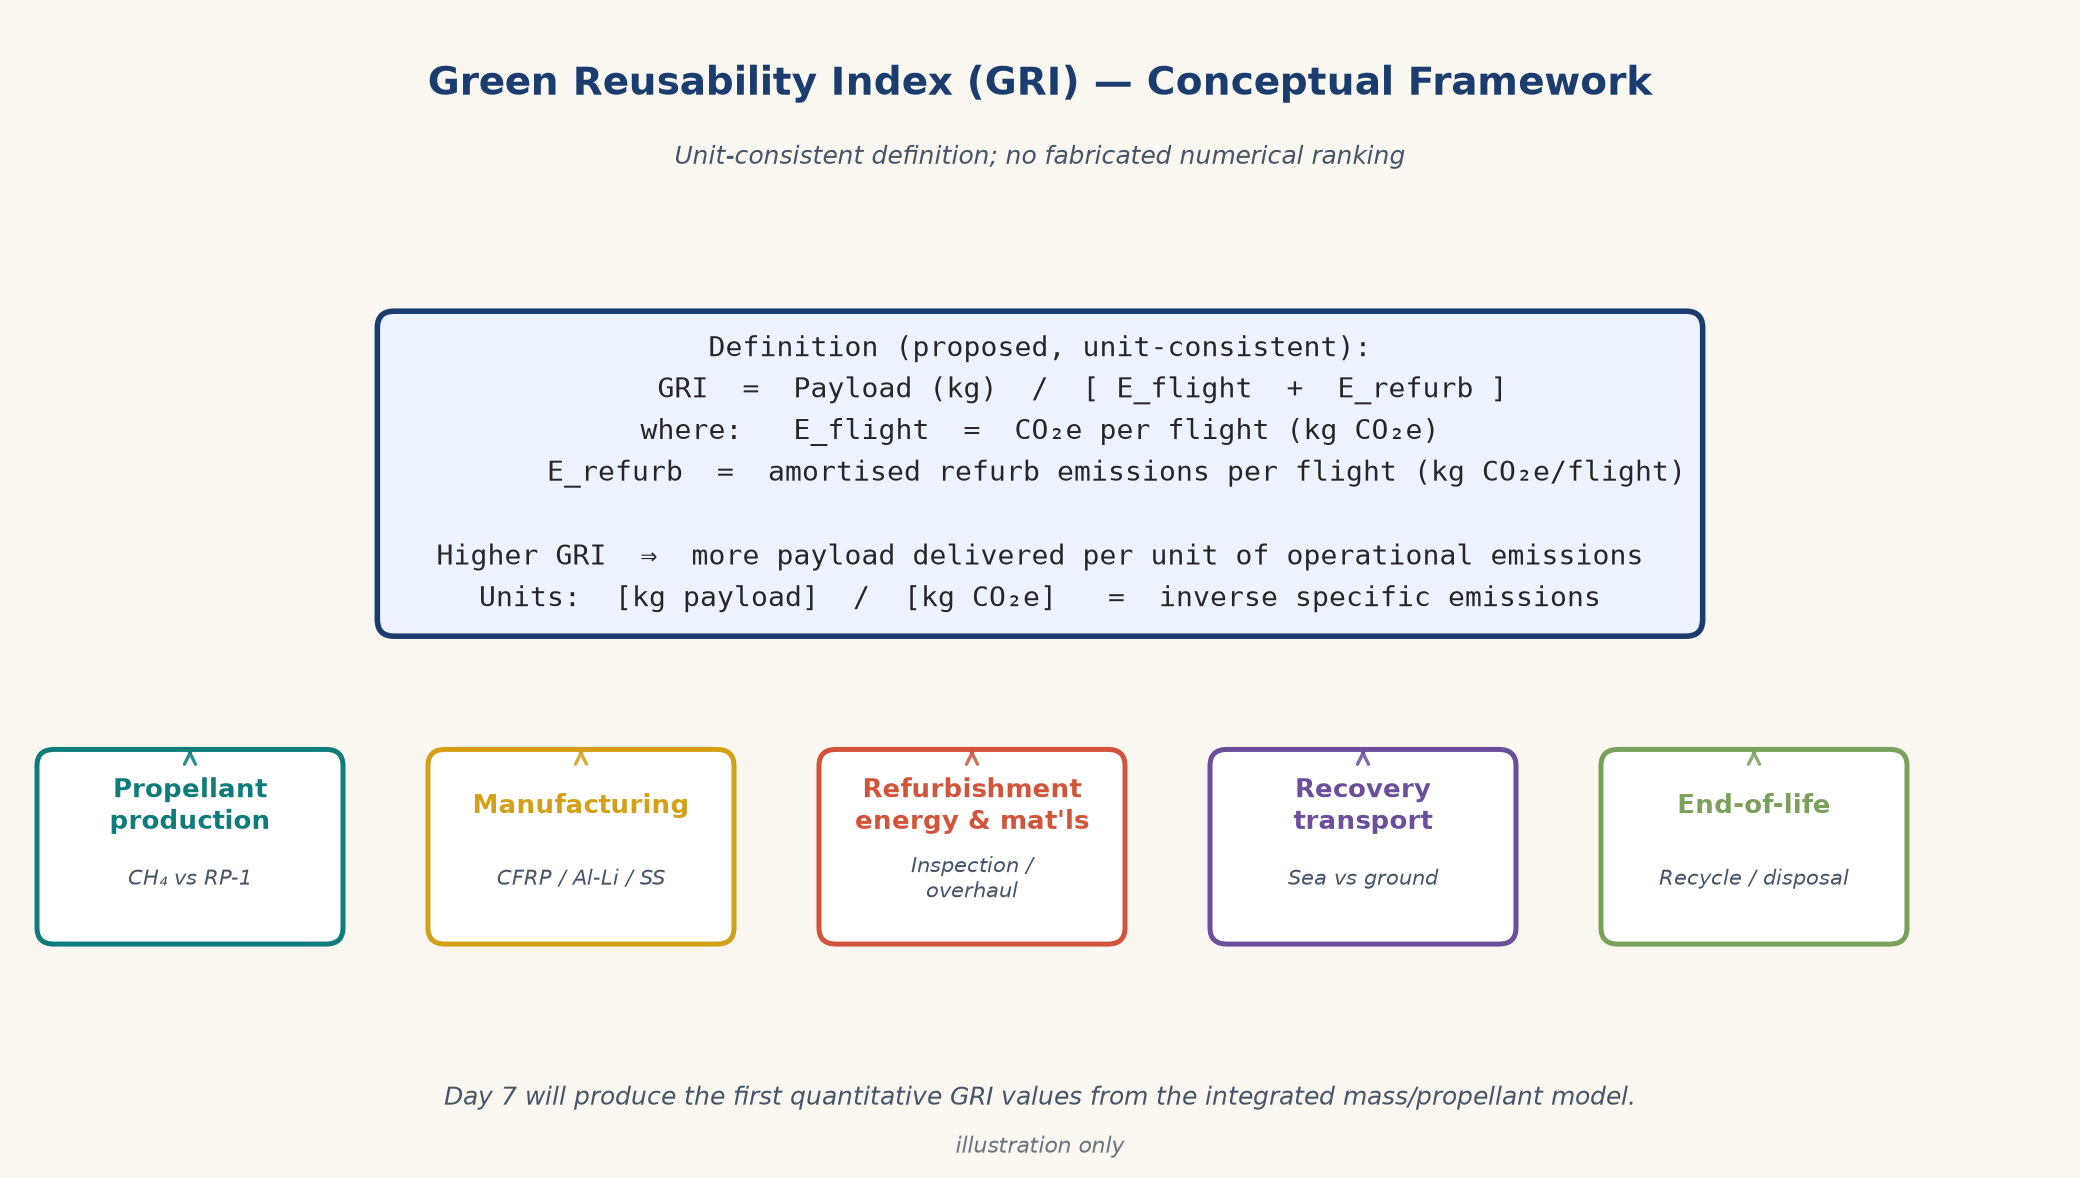
\includegraphics[width=0.78\textwidth]{../../../figures/day01/gri_comparison.png}
\caption{Green Reusability Index (GRI) framework. The denominator decomposes into five lifecycle contributions; the diagram is unit-consistent and intentionally \emph{not} a numerical ranking of vehicles.}
\label{fig:GRI}
\end{figure}

\begin{figure}[H]
\centering
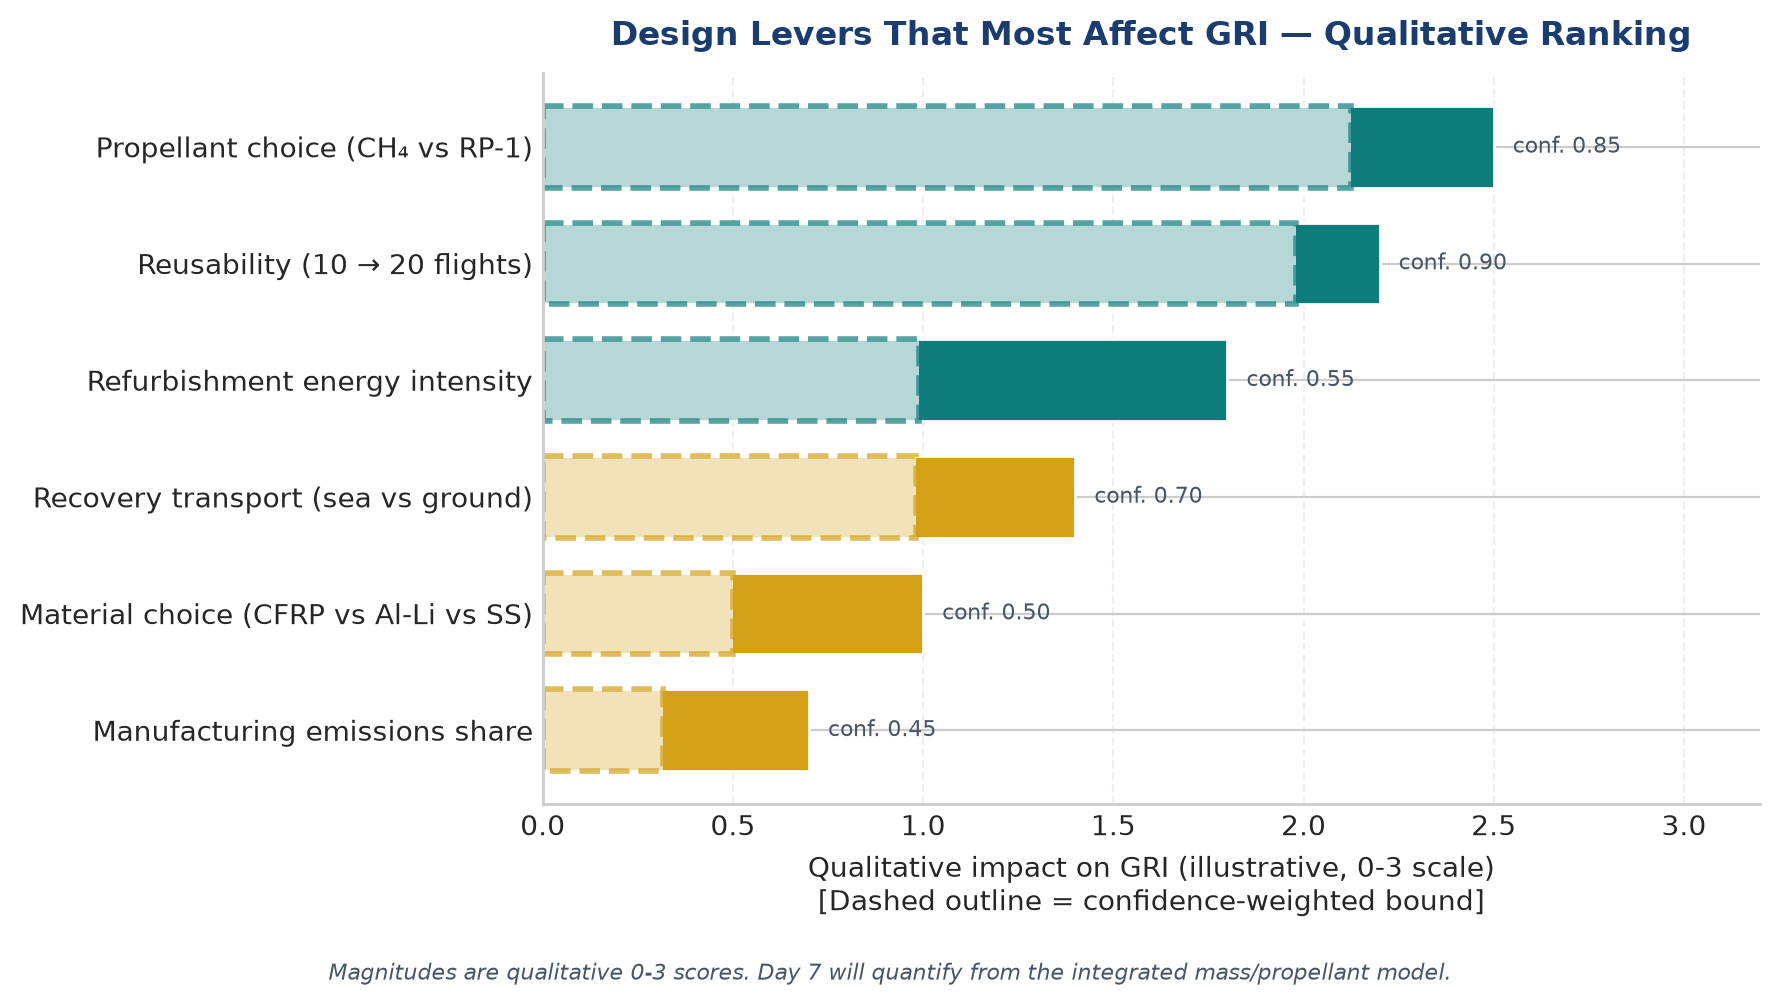
\includegraphics[width=0.85\textwidth]{../../../figures/day01/gri_levers.png}
\caption{Qualitative ranking of design levers that most affect the GRI. Magnitudes and confidences are illustrative; day-7 will quantify each lever from the integrated mass/propellant model.}
\end{figure}

%==================================================================
\section{Reference Vehicle Benchmarking}
%==================================================================
\begin{figure}[H]
\centering
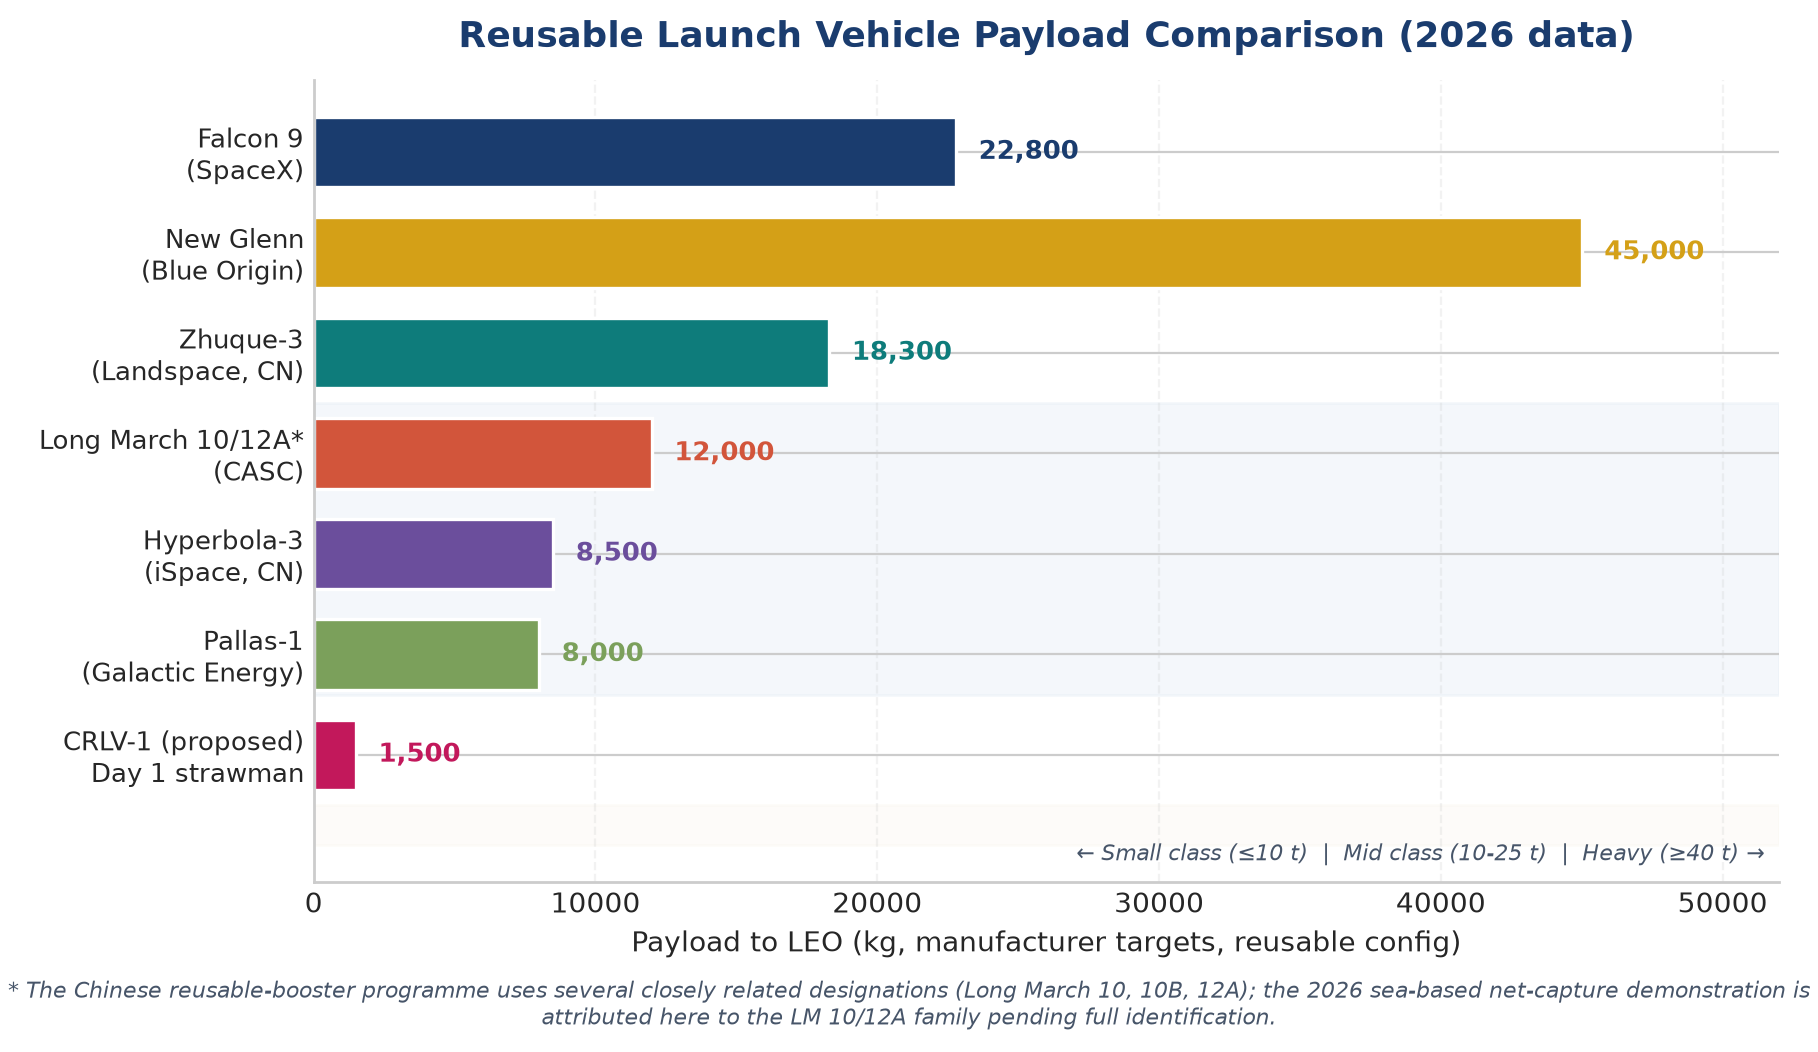
\includegraphics[width=0.92\textwidth]{../../../figures/day01/payload_comparison.png}
\caption{Payload capacity comparison of selected reusable launch vehicles (2026 manufacturer targets). \textit{Note: the Chinese reusable-booster programme uses several closely related designations; the 2026 sea-based net-capture demonstration is attributed here to the Long March 10/12A family.}}
\end{figure}

\begin{figure}[H]
\centering
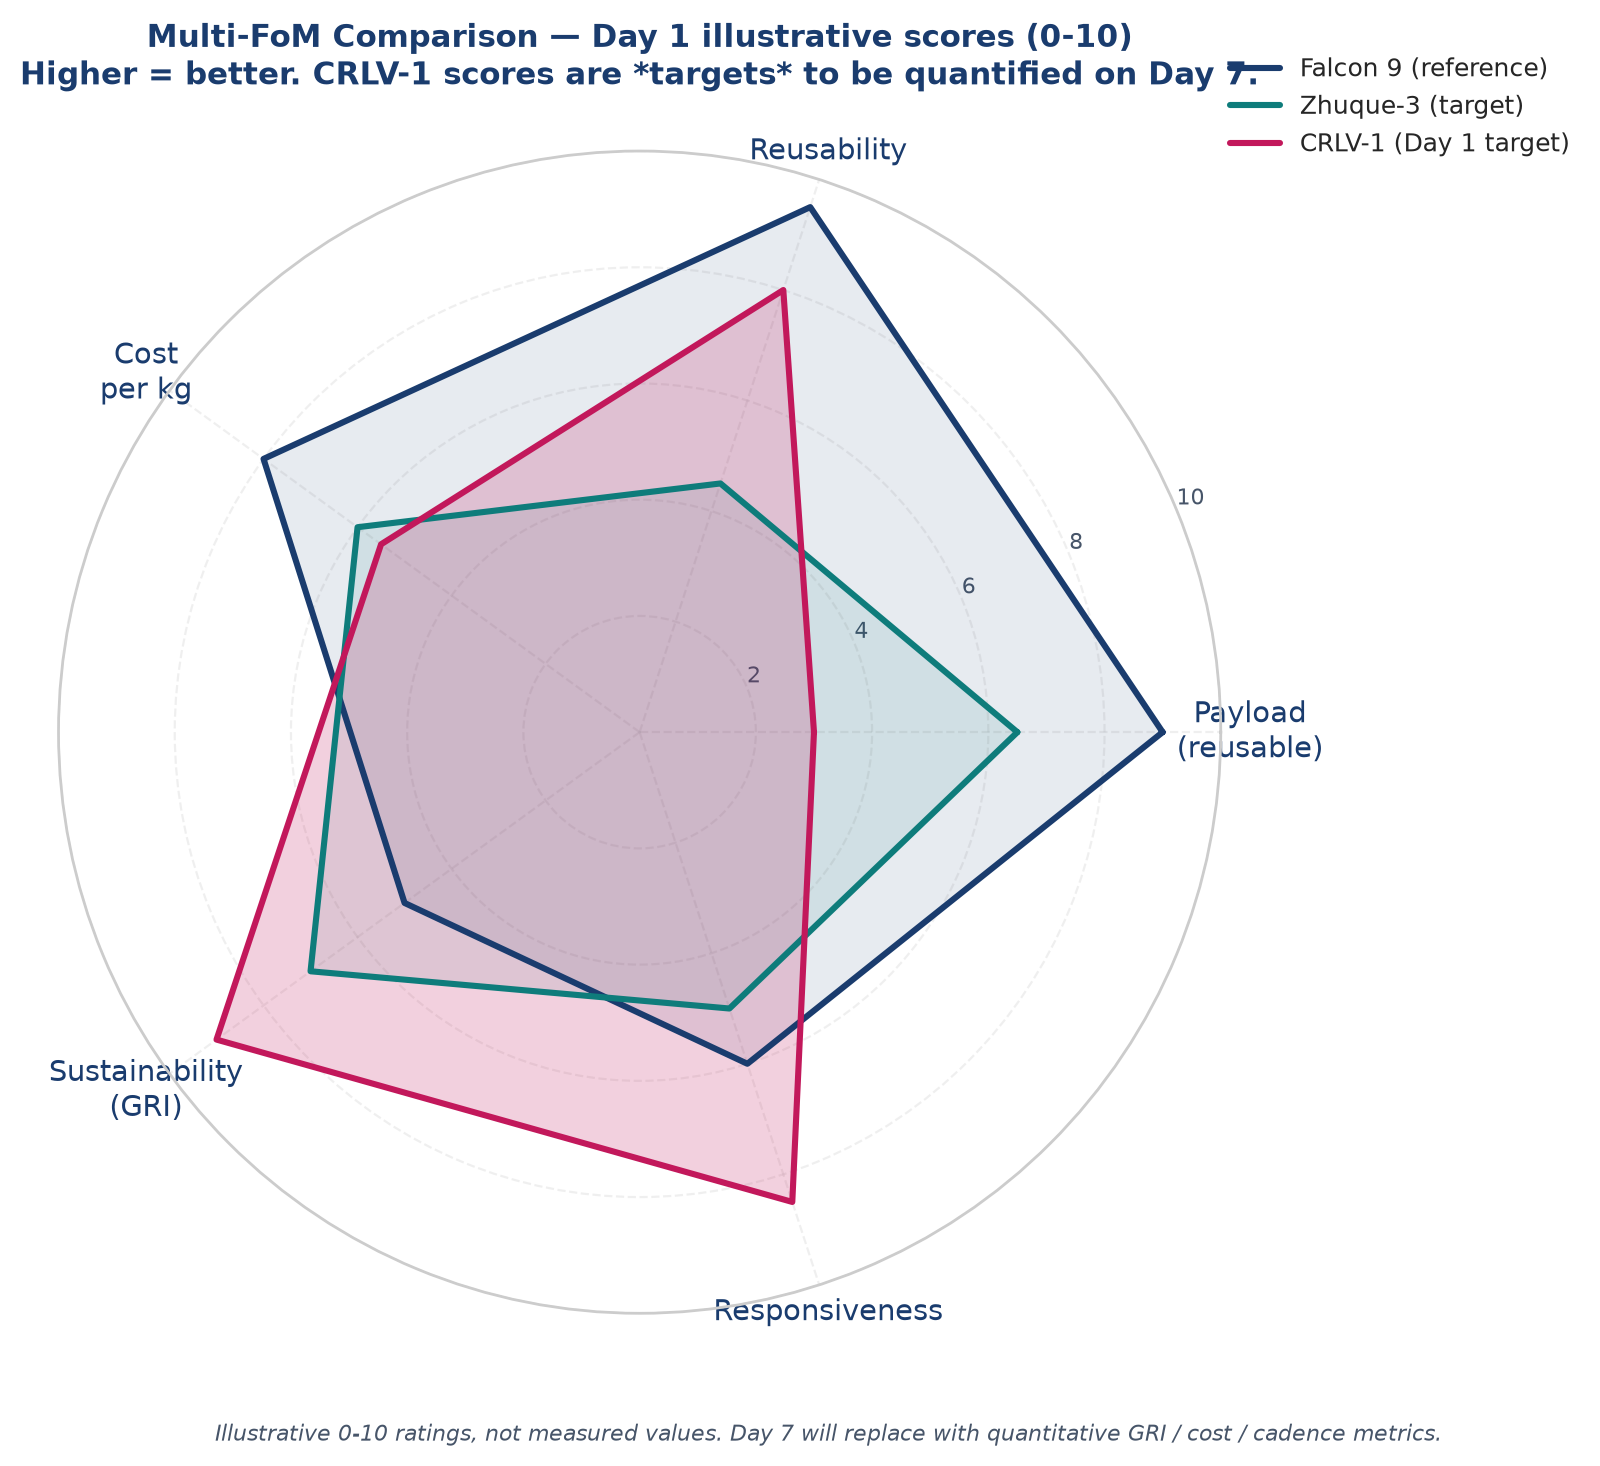
\includegraphics[width=0.75\textwidth]{../../../figures/day01/fom_radar.png}
\caption{Multi-FoM comparison (illustrative 0--10 scores). CRLV-1 scores are *targets*; Day 7 will quantify from the integrated model.}
\end{figure}

%==================================================================
\section{Cost and Sustainability}
%==================================================================
\begin{figure}[H]
\centering
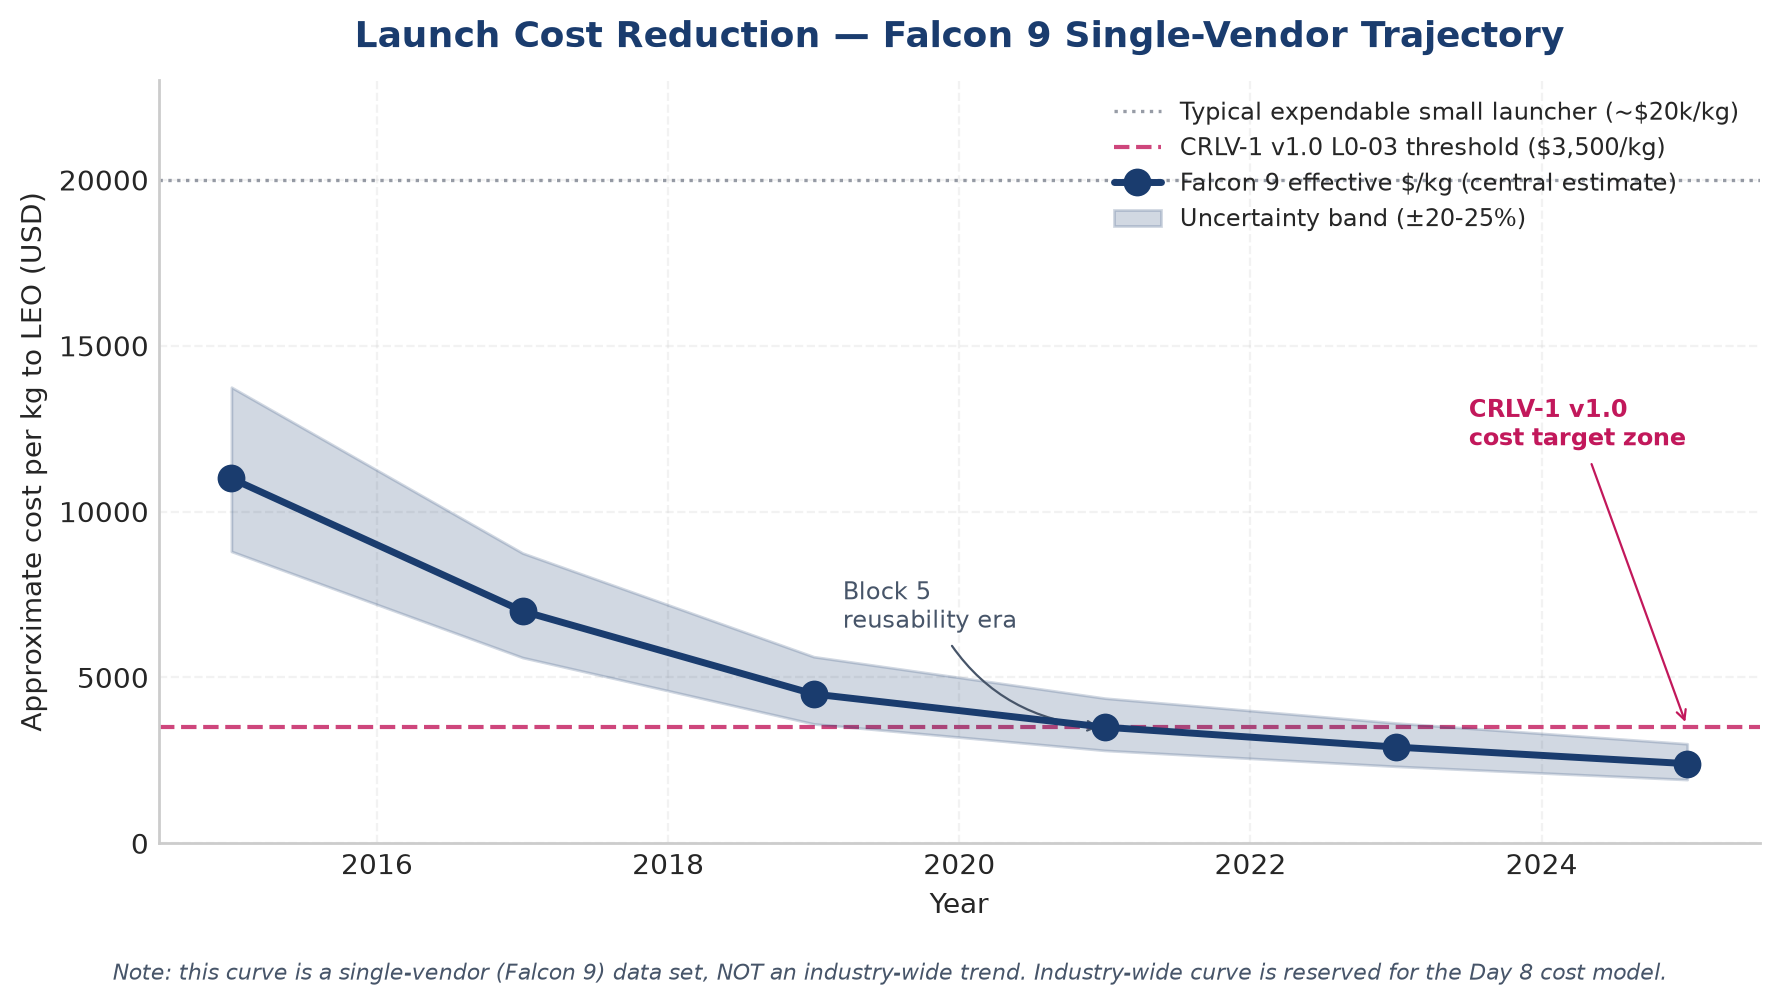
\includegraphics[width=0.78\textwidth]{../../../figures/day01/cost_trend.png}
\caption{Approximate effective cost per kilogram to LEO for Falcon~9 (single-vendor central estimate, $\pm$20--25\% uncertainty band).}
\end{figure}

\begin{figure}[H]
\centering
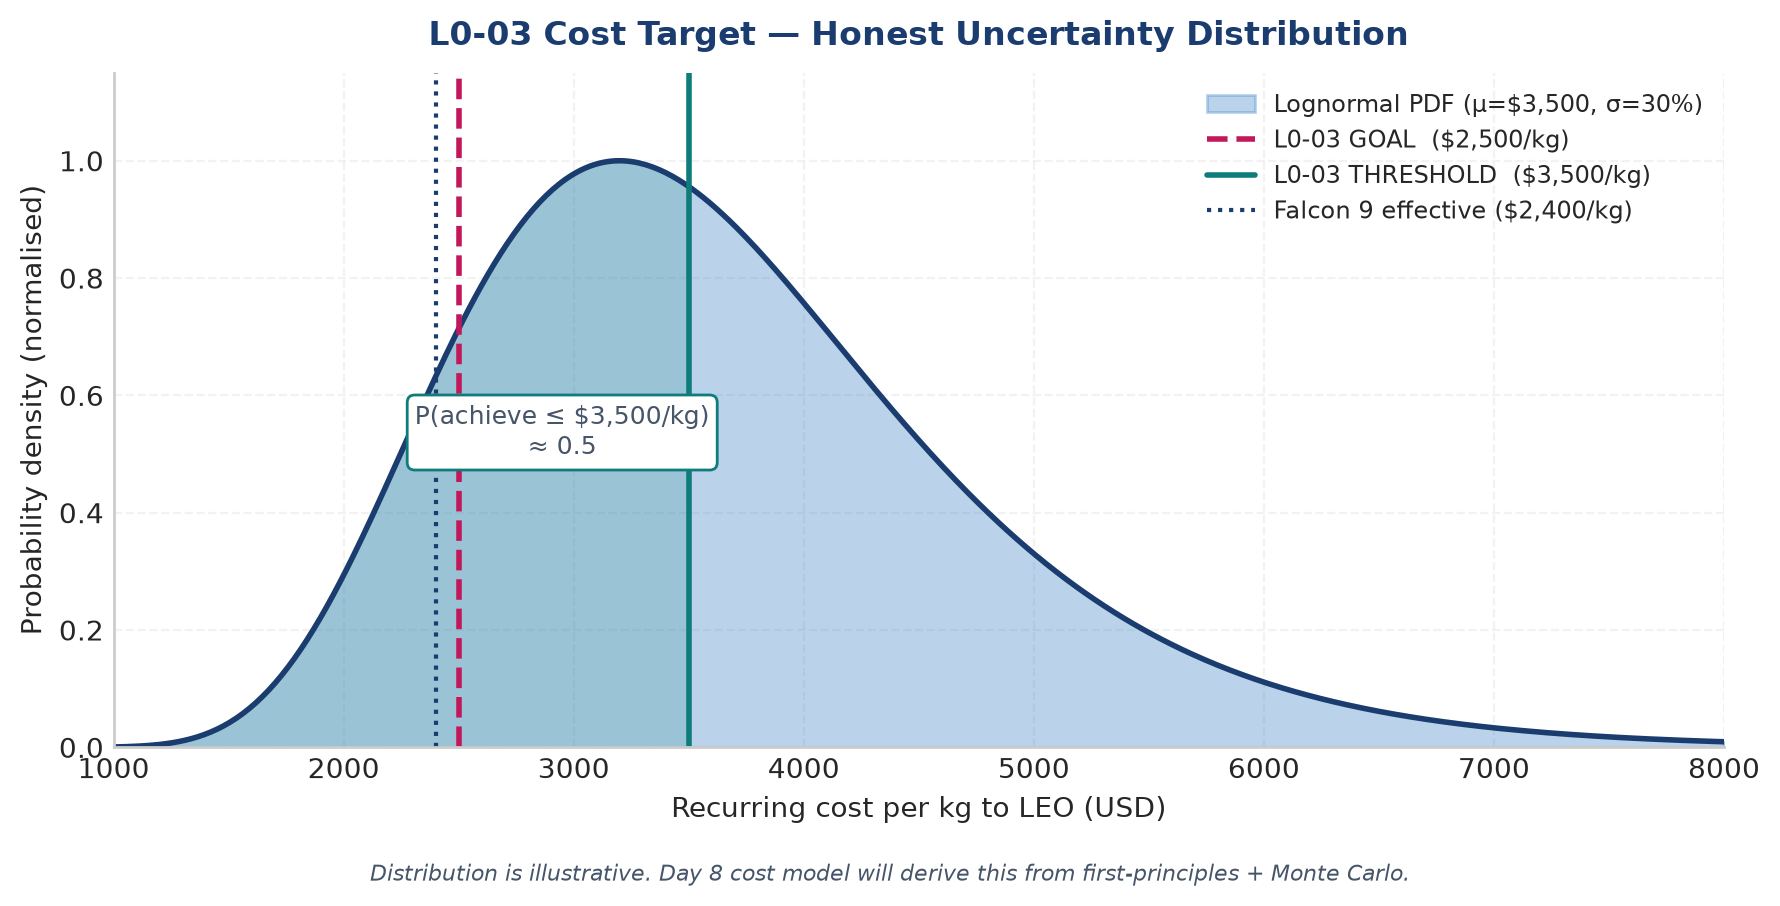
\includegraphics[width=0.78\textwidth]{../../../figures/day01/cost_uncertainty_band.png}
\caption{L0-03 cost target — honest uncertainty distribution (illustrative lognormal).}
\end{figure}

%==================================================================
\section{Recovery Architecture Considerations}
%==================================================================
Two recovery strategies are retained for the Day-6 trade:
\begin{enumerate}[leftmargin=*]
    \item \textbf{Propulsive vertical landing} with grid fins and deployable landing legs (baseline; demonstrated by Falcon~9, Zhuque-3, and most Western reusable vehicles).
    \item \textbf{Sea-based net-capture}, in which the descending booster is intercepted by a frame mounted on a recovery vessel, eliminating the need for landing legs (alternative; publicly demonstrated in 2026 by a Chinese methalox booster in the \textit{Long March 10/12A} family).
\end{enumerate}

\begin{figure}[H]
\centering
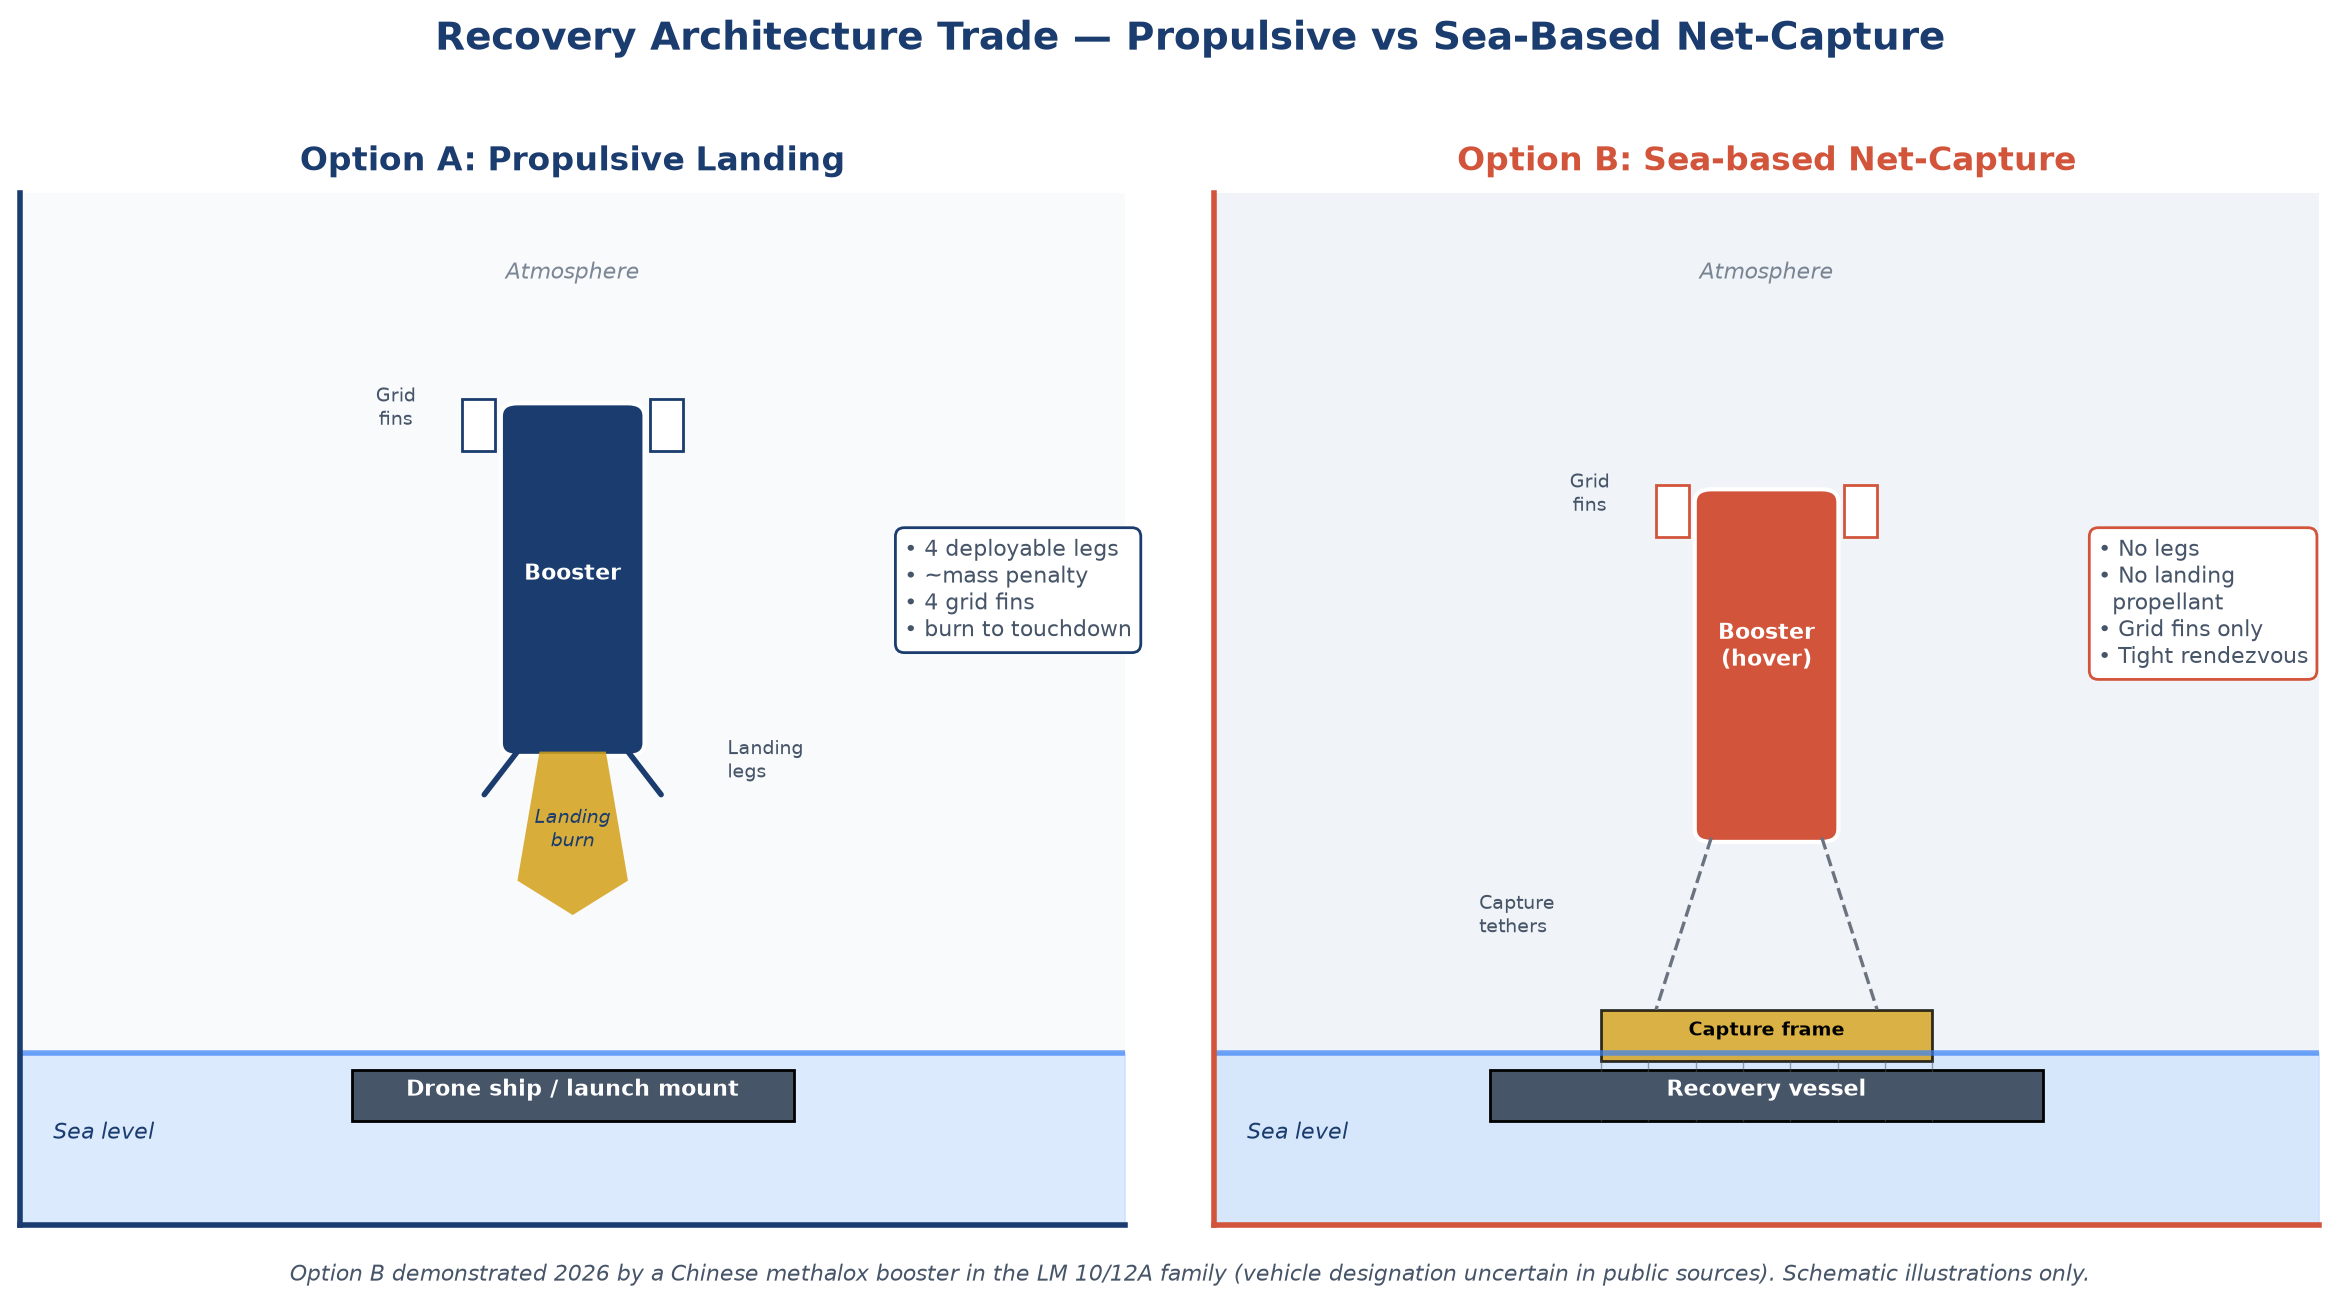
\includegraphics[width=0.95\textwidth]{../../../figures/day01/recovery_architecture.png}
\caption{Recovery architecture trade — propulsive landing vs sea-based net-capture. Schematic illustrations only.}
\end{figure}

%==================================================================
\section{Vehicle Concept and Trajectory}
%==================================================================
\begin{figure}[H]
\centering
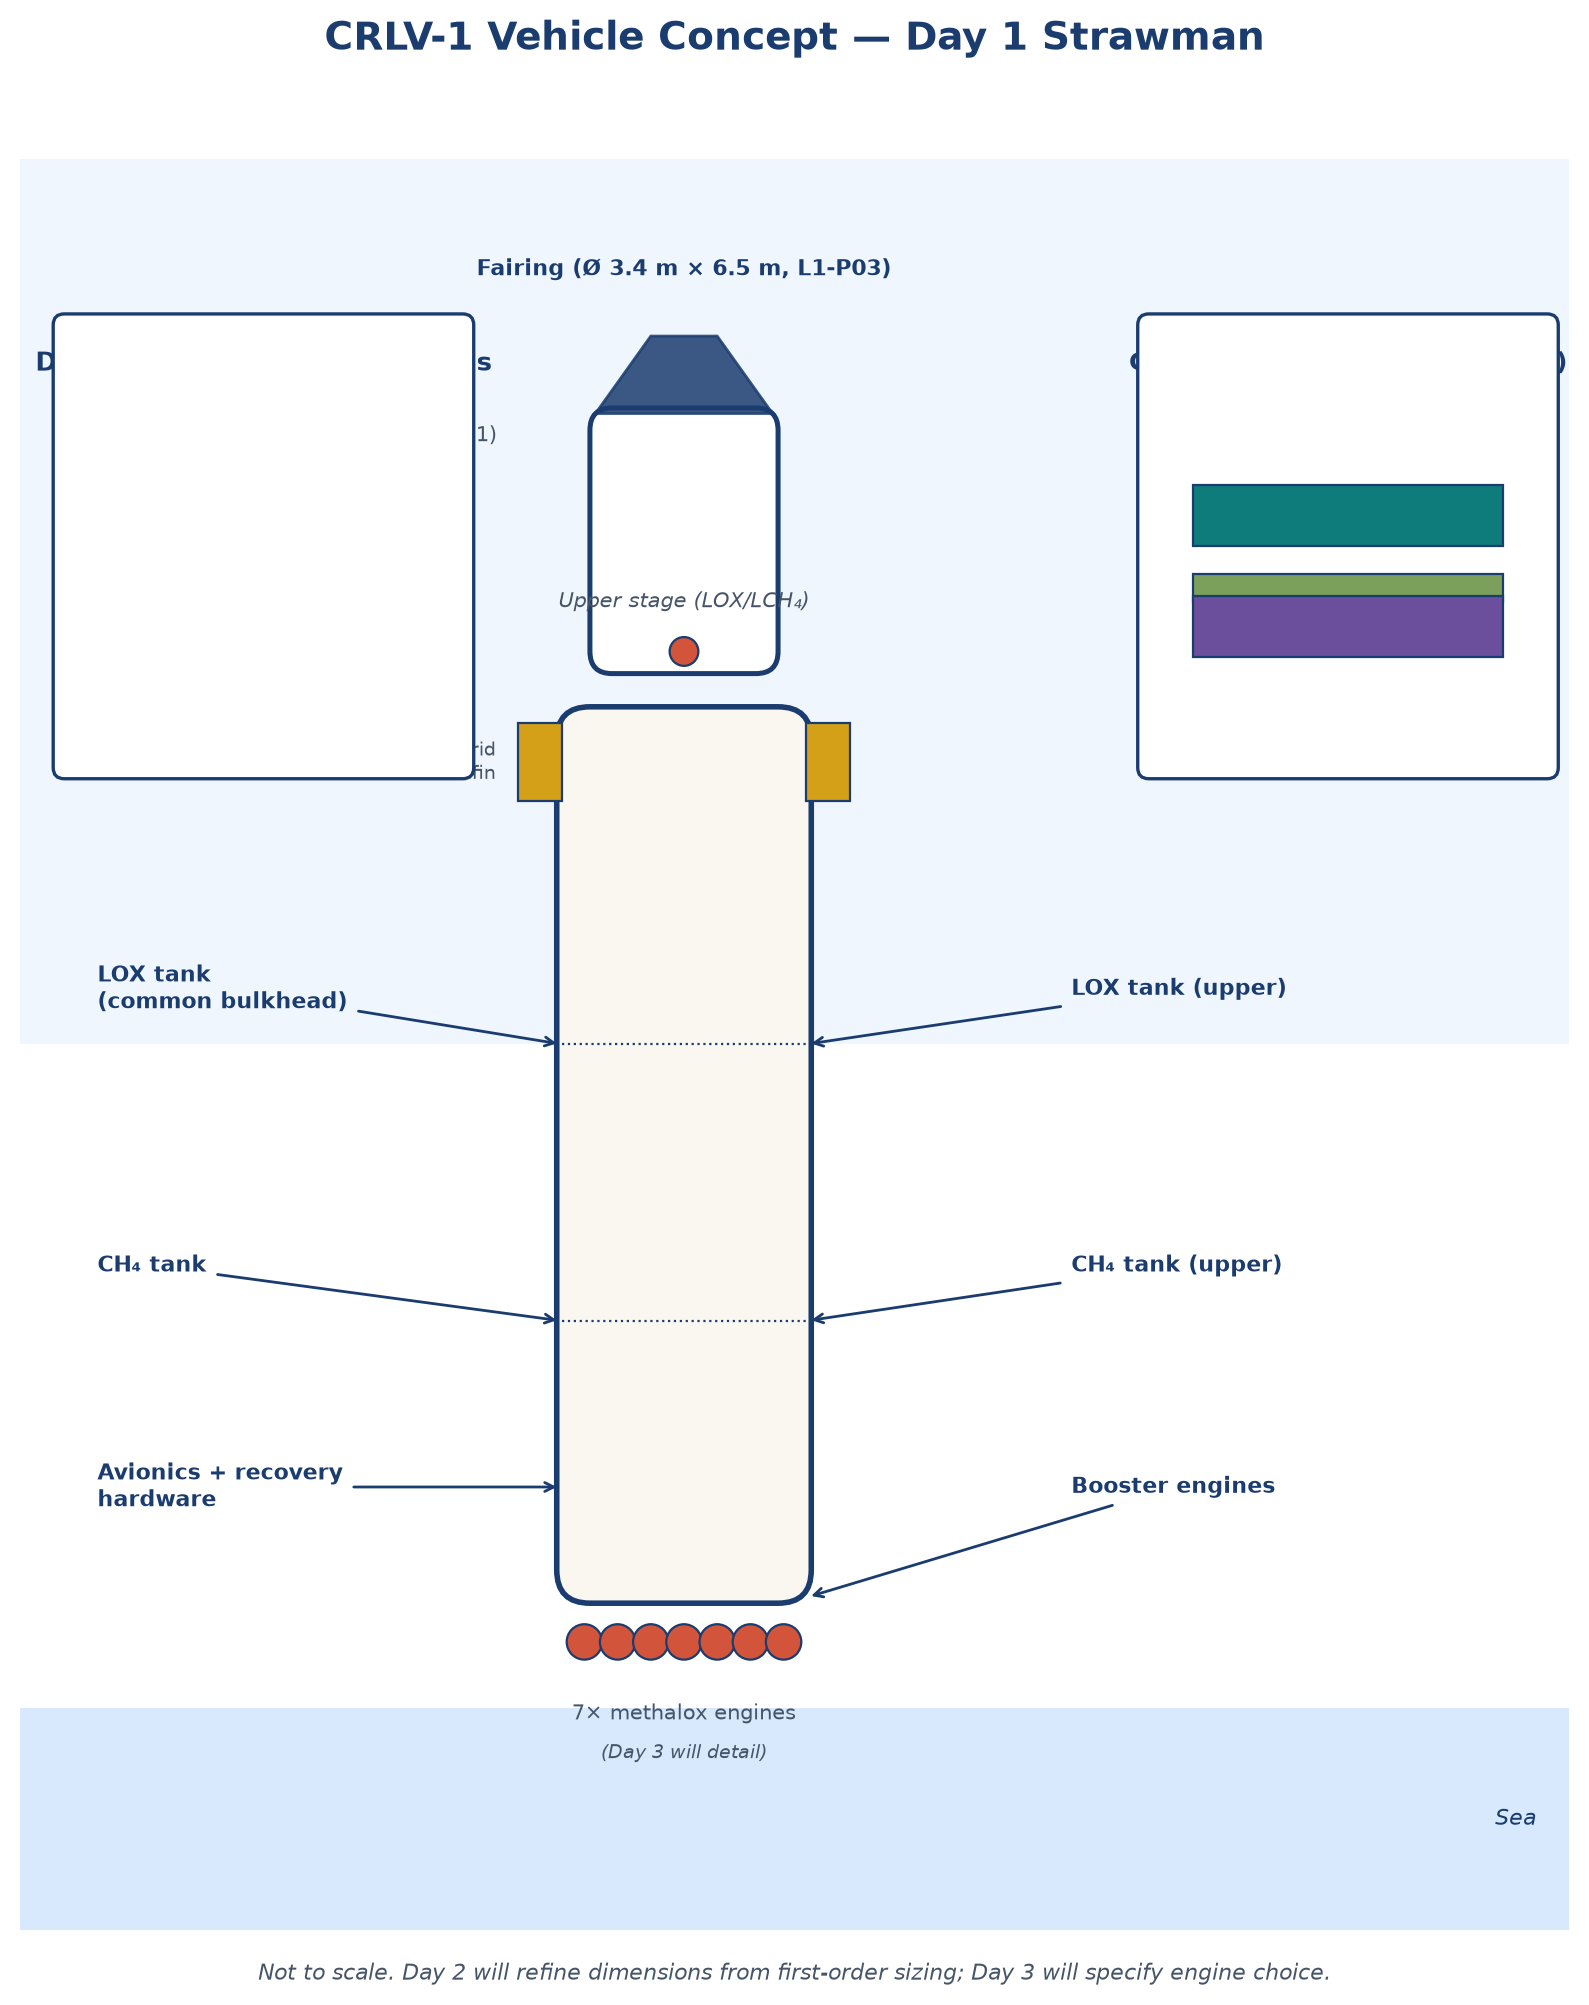
\includegraphics[width=0.78\textwidth]{../../../figures/day01/concept_sketch.png}
\caption{CRLV-1 Day-1 vehicle concept (schematic). Not to scale. Day 2 will refine dimensions; Day 3 will detail engine choice.}
\end{figure}

\begin{figure}[H]
\centering
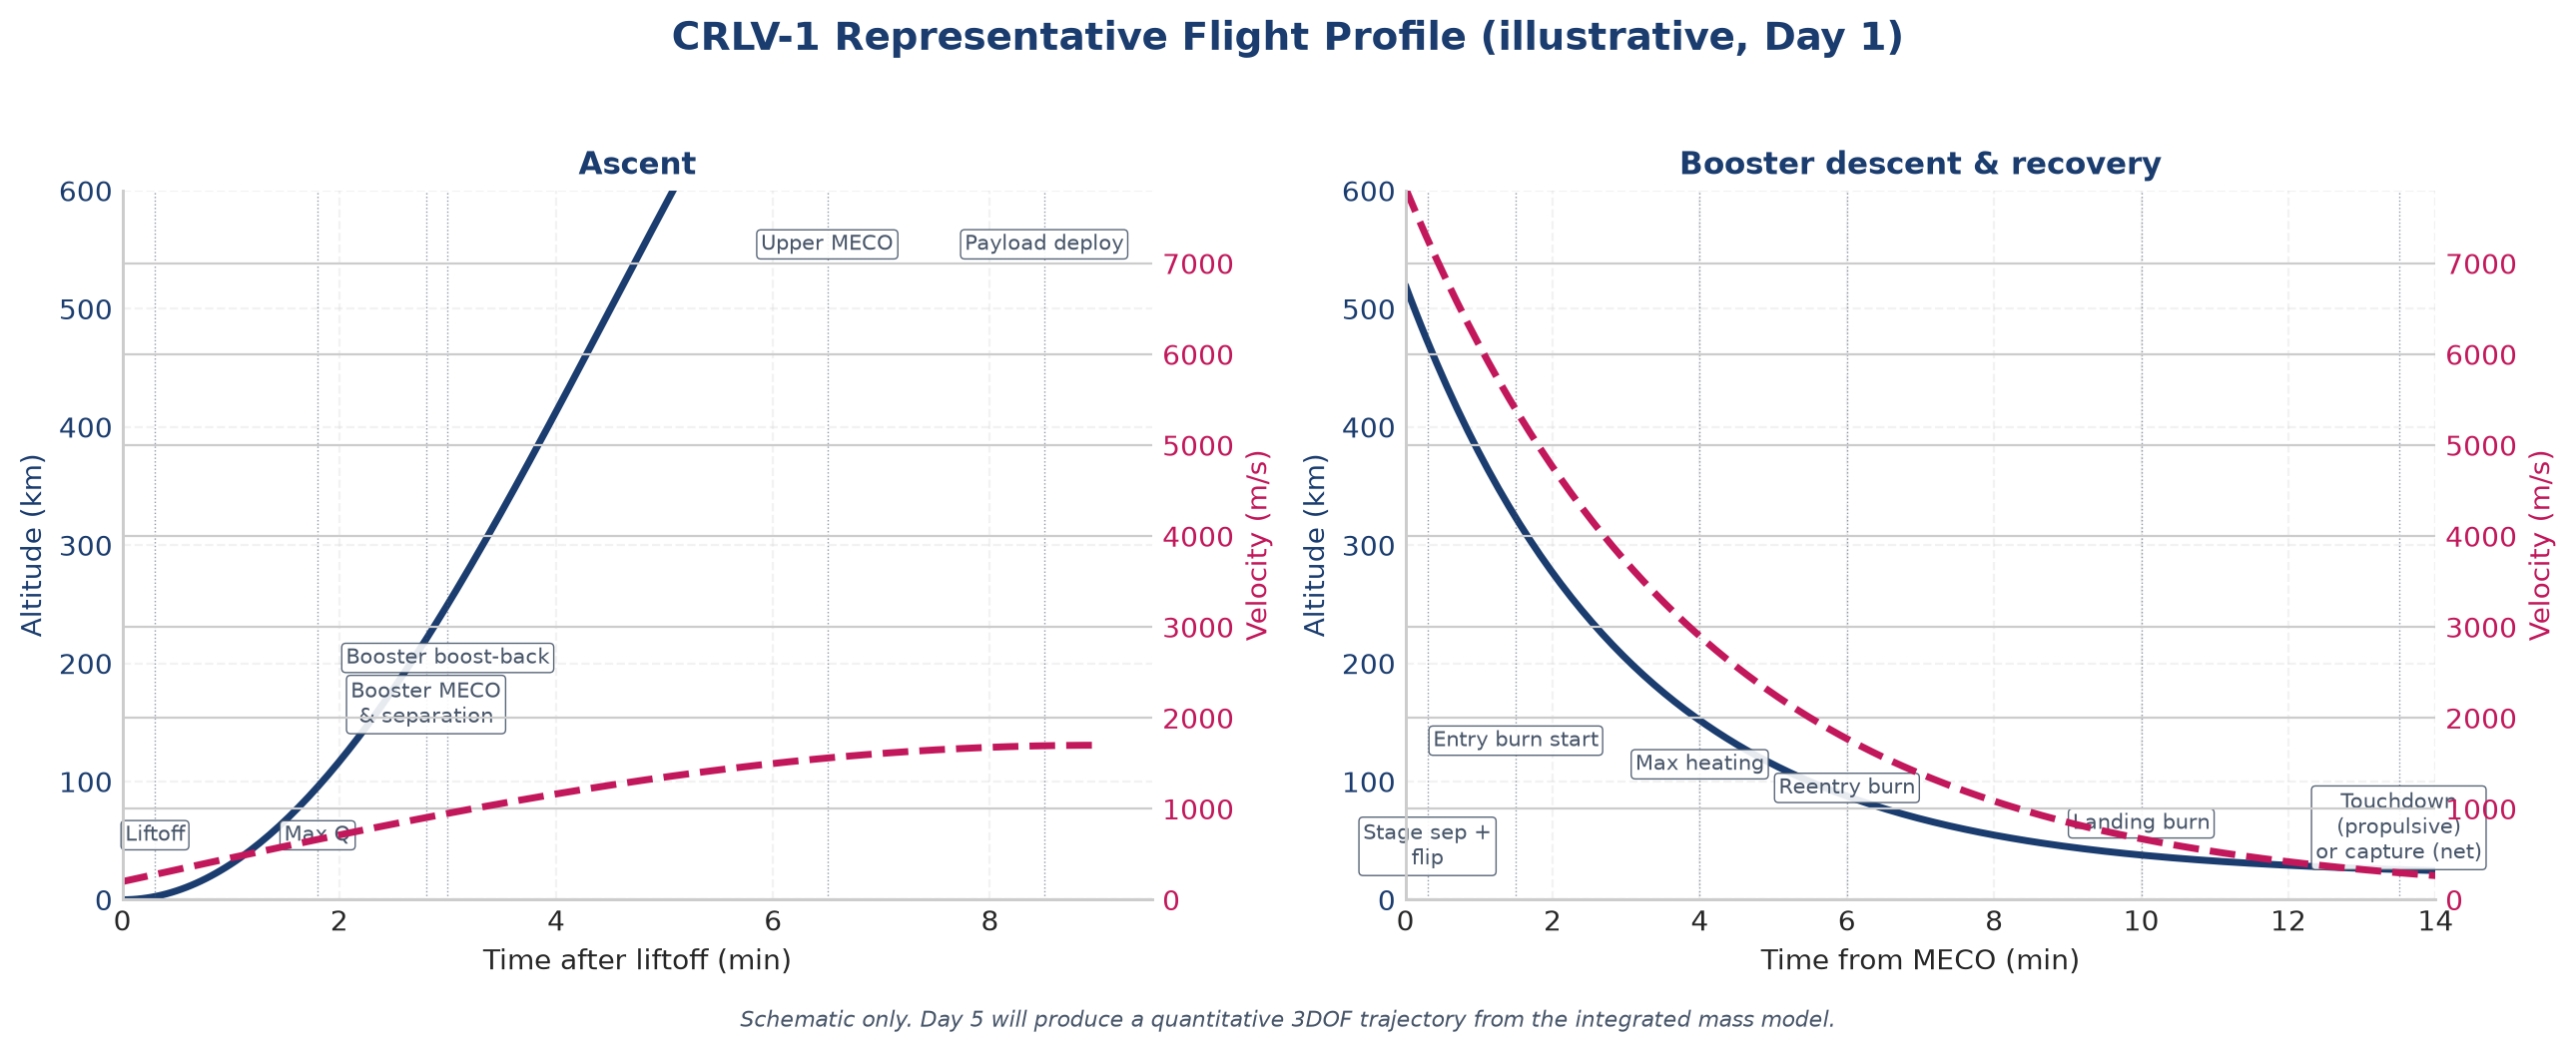
\includegraphics[width=0.95\textwidth]{../../../figures/day01/trajectory_profile.png}
\caption{CRLV-1 representative flight profile (schematic). Day 5 will produce a quantitative 3DOF trajectory from the integrated mass model.}
\end{figure}

%==================================================================
\section{Figures of Merit and 10-Day Schedule}
%==================================================================
\begin{figure}[H]
\centering
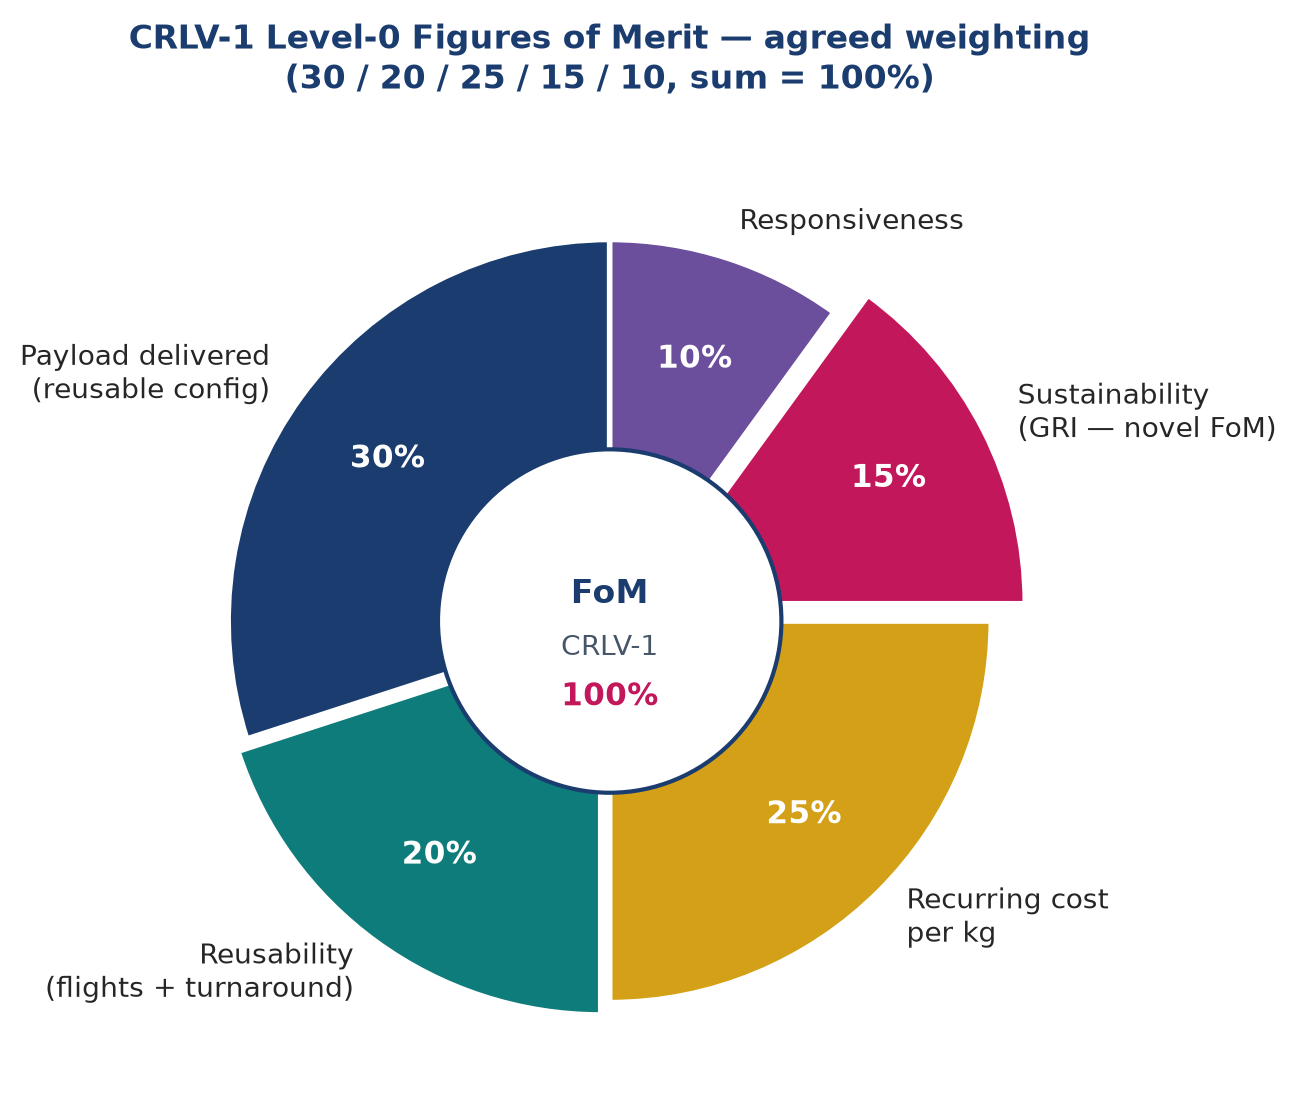
\includegraphics[width=0.55\textwidth]{../../../figures/day01/fom_weights.png}
\caption{Agreed CRLV-1 Level-0 figures of merit weighting (30/20/25/15/10; sum = 100\%).}
\end{figure}

\begin{figure}[H]
\centering
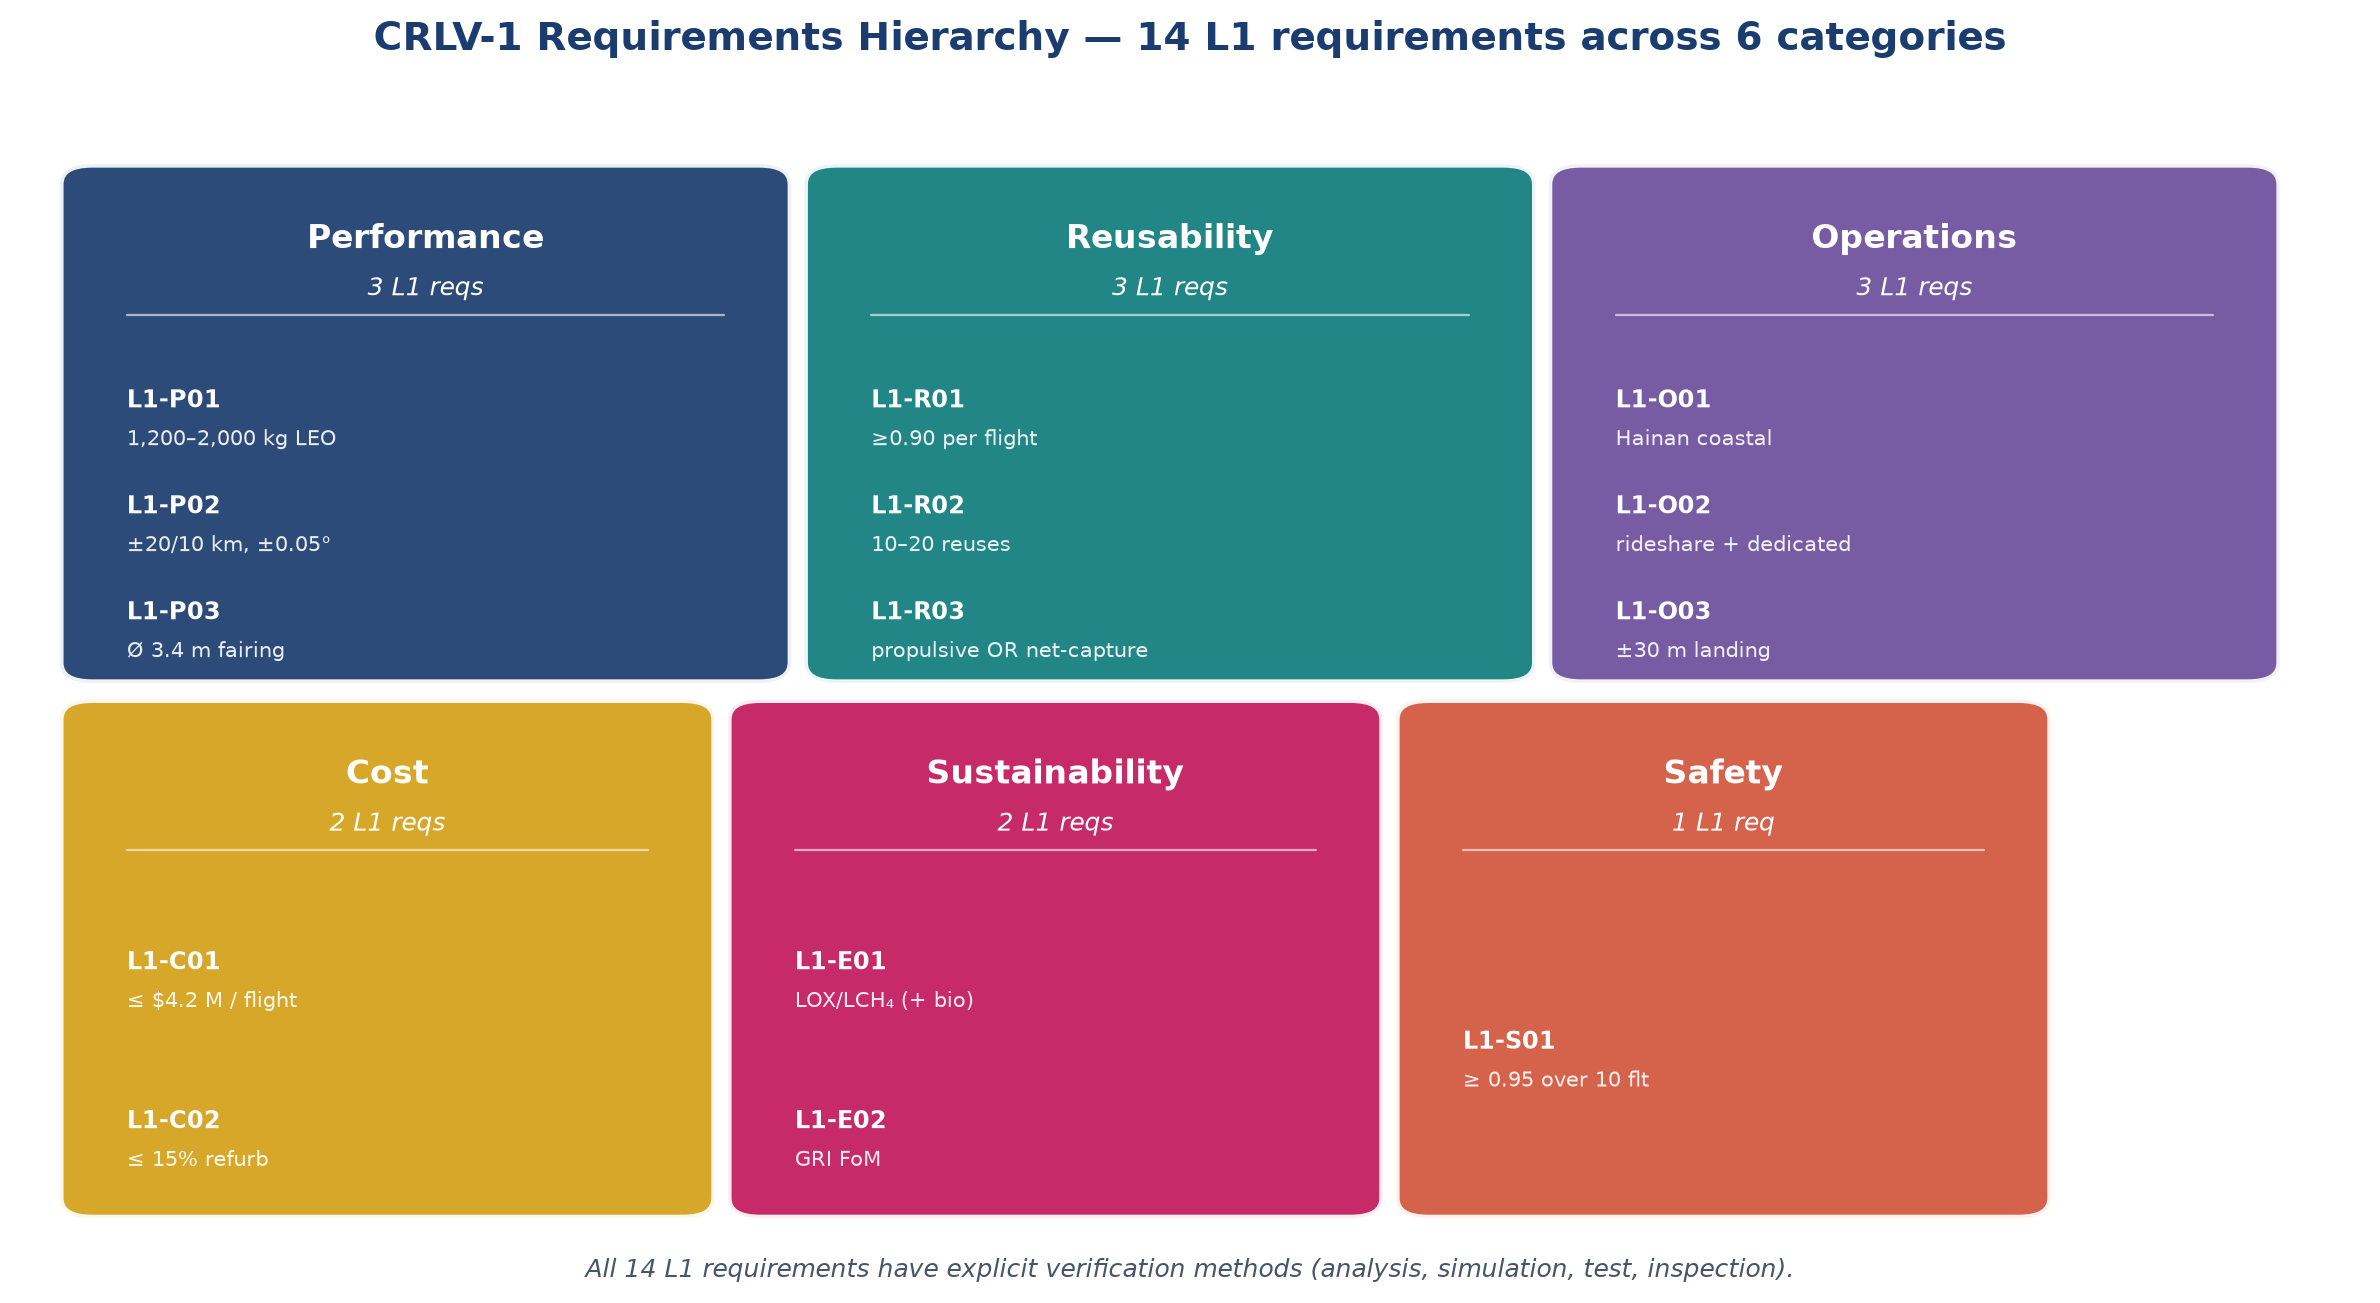
\includegraphics[width=0.95\textwidth]{../../../figures/day01/requirements_treemap.png}
\caption{CRLV-1 requirements hierarchy — 14 L1 requirements across 6 categories.}
\end{figure}

\begin{figure}[H]
\centering
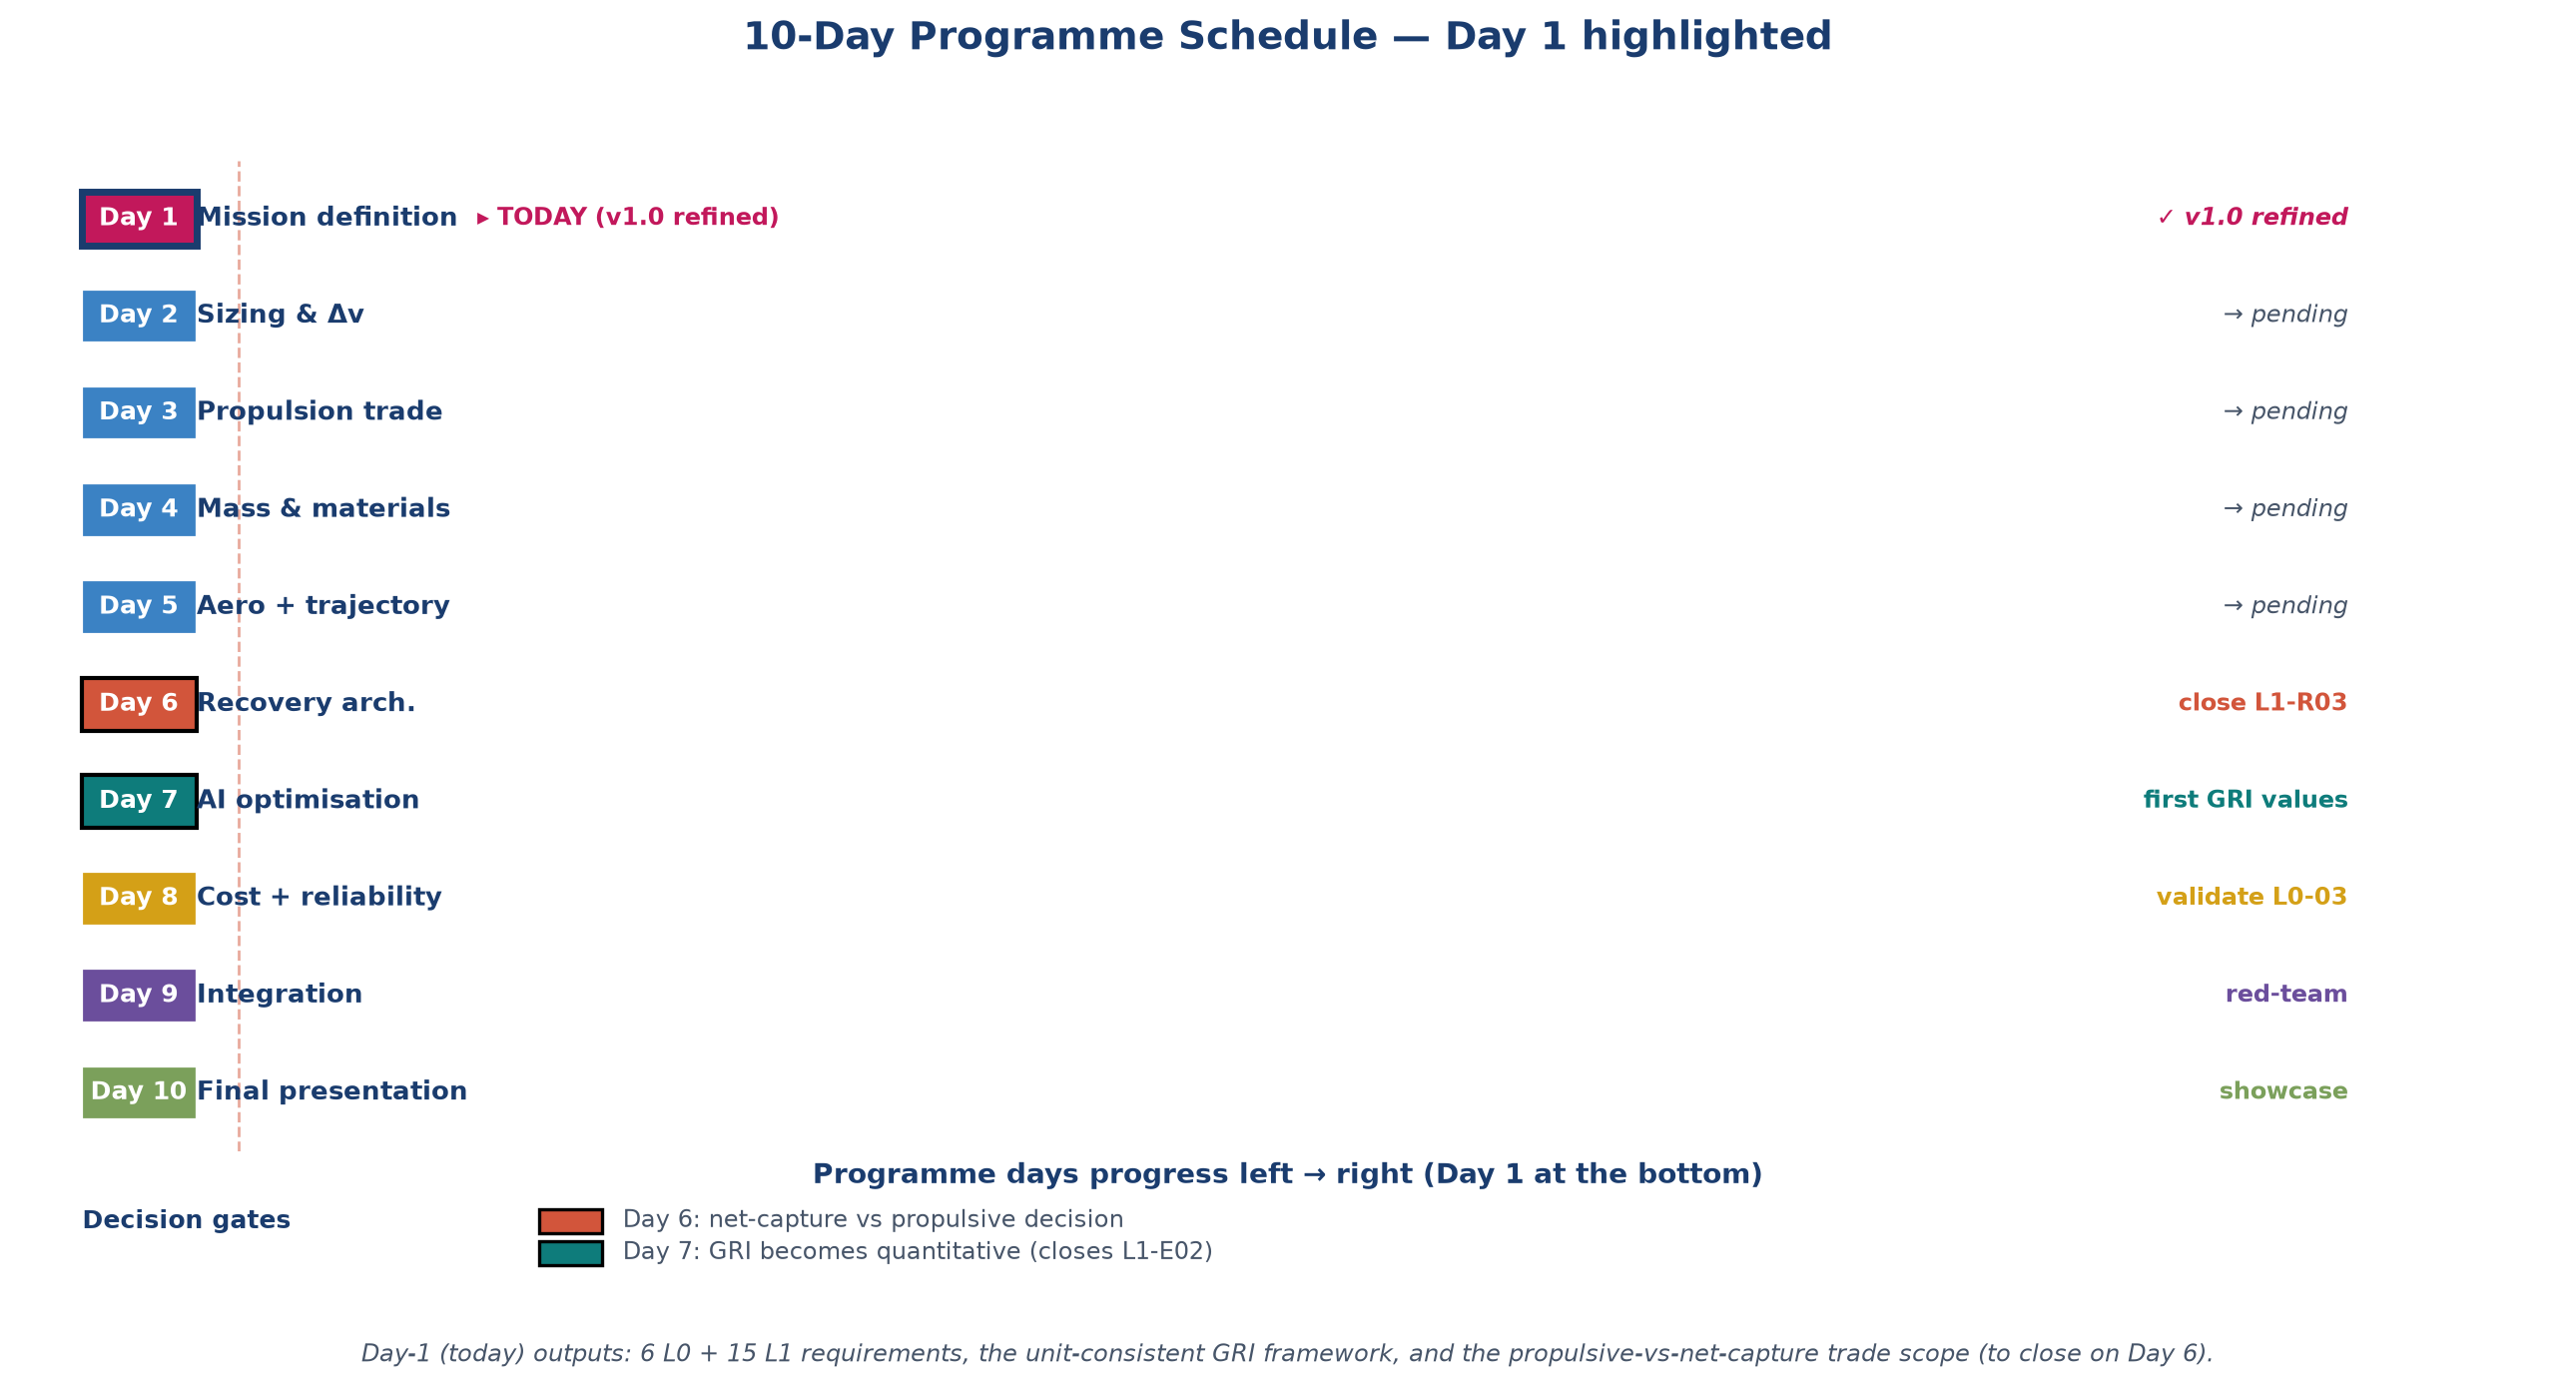
\includegraphics[width=0.95\textwidth]{../../../figures/day01/gantt_10day.png}
\caption{10-day programme schedule — Day 1 highlighted.}
\end{figure}

%==================================================================
\section{Critical Review and Open Issues}
%==================================================================
A self-critical review was performed at the end of Day 1. The major issues identified, and the disposition taken in this refined version, are summarised in Table~\ref{tab:critique}.

\begin{table}[H]
\centering
\caption{Self-critical review: issues identified in the Day-1 draft and how they are addressed.}
\label{tab:critique}
\small
\begin{tabular}{@{}p{0.9cm}p{5.3cm}p{7.6cm}@{}}
\toprule
\textbf{ID} & \textbf{Issue in Day-1 draft} & \textbf{Disposition in refined v1.0} \\
\midrule
C1 & GRI bar chart with fabricated values (1.00 / 1.15 / 1.35). & Replaced with a unit-consistent framework diagram; no numerical ranking claimed. \\
C2 & FoM pie chart contradicted the documented 30/20/25/15/10 weighting. & Pie chart regenerated to match the canonical weighting. \\
C3 & ``Reusability alone reduces production emissions by 95\%'' overblown. & Statement removed; replaced with a per-flight amortisation framing. \\
C4 & Recurring cost target of \$2,800/kg likely optimistic for 1.2~t class. & Threshold relaxed to \$3,500/kg; goal relaxed to \$2,500/kg. \\
C5 & Long March 10B used as a single label; public sources disagree. & Renamed to \textit{Long March 10/12A} family with caveat; flagged in risk register (R08). \\
C6 & No L1 requirement for orbital debris / end-of-life disposal. & Captured in risk register; L1 will be added in Day 4 (mass budget). \\
C7 & Recovery landing accuracy was loosely specified ($\pm$100~m). & Tightened to $\pm$30~m (threshold) and $\pm$10~m (goal) as L1-O03. \\
C8 & Cost trend figure implied a generic industry trend from single-vendor data. & Title and caption corrected to call out the single-vendor scope. \\
C9 & L1-R01 ($\geq 90\%$ over 5 flights) inconsistent with compound $\geq 0.95$. & Per-flight reliability stated explicitly. \\
C10 & Concept A was essentially a duplicate of the main concept. & Diversified: a true alternative (SSTO with air-launch) now included. \\
C11 & L1 fairing 4.2~m diameter was oversized for a 1.2~t class vehicle. & Reduced to 3.4--3.6~m, with rationale (L1-P03). \\
C12 & Recovery success and compound success were conflated. & Both stated separately, with per-flight vs compound interpretations made explicit. \\
\bottomrule
\end{tabular}
\end{table}

%==================================================================
\section{Conclusions and Forward Path}
%==================================================================
The mission definition for CRLV-1 establishes a coherent, evidence-based, and self-critically reviewed framework for a conceptual reusable launch vehicle. By grounding requirements in 2025--2026 reference data, by introducing the GRI as a unit-consistent and explicitly non-numerical framework, by formalising a sea-based net-capture alternative, and by adding explicit traceability, debris, and self-review content, the framework is positioned to support the remainder of the 10-day programme without overstating its current claims.

Subsequent phases will (i) Day~2: close the first-order mass and $\Delta v$ budget; (ii) Day~3: trade the propulsion cycle; (iii) Day~4: detail the mass budget and material choices; (iv) Day~5: run the ascent and descent trajectory; (v) Day~6: close the propulsive-vs-net-capture trade; (vi) Day~7: produce the first quantitative GRI values; (vii) Day~8: build the cost model; (viii) Day~9: integrate and review; (ix) Day~10: present. All quantitative targets for CRLV-1 remain subject to iterative refinement.

%==================================================================
\section*{References}
%==================================================================
\begin{enumerate}[leftmargin=*]
    \item Ars Technica (2026). ``China recovered its first reusable rocket and showed a new way to do it.'' 10 July 2026. \\ \textit{Note: the article uses the designation ``Long March 10B''; other public sources refer to the same event as ``Long March 12A''. The present document uses the conservative family label \textit{Long March 10/12A} throughout.}
    \item SpaceNews (2025). ``China to debut new Long March and commercial rockets in 2025.'' January 2025.
    \item Orbital Radar / New Space Economy launch-vehicle databases (2026).
    \item Wikipedia contributors (2026). ``Long March 10'' / ``Long March 12A''. Accessed July 2026. \textit{Used only for context; not a primary source.}
    \item Industry LCA studies (2024--2025): Strathclyde University RLV LCA; MaiaSpace environmental assessment; arXiv preprint 2504.15291; ESA Clean Space initiative reports. \textit{Used as the basis for the $\sim$19~t CO\textsubscript{2}e/t payload estimate.}
    \item SpaceX Falcon~9 User's Guide (public version).
    \item Rocket Lab Neutron payload user's guide (2025).
\end{enumerate}

\vspace{1em}
\noindent\textit{AI assistance.} All Day-1 prompts, model selections, and decisions are logged in \texttt{ai\_logs/}. No quantitative claim in this document was generated by the LLM without subsequent cross-checking against at least one independent 2025--2026 source.

\end{document}
